\section{Полиномиальное хеширование.}
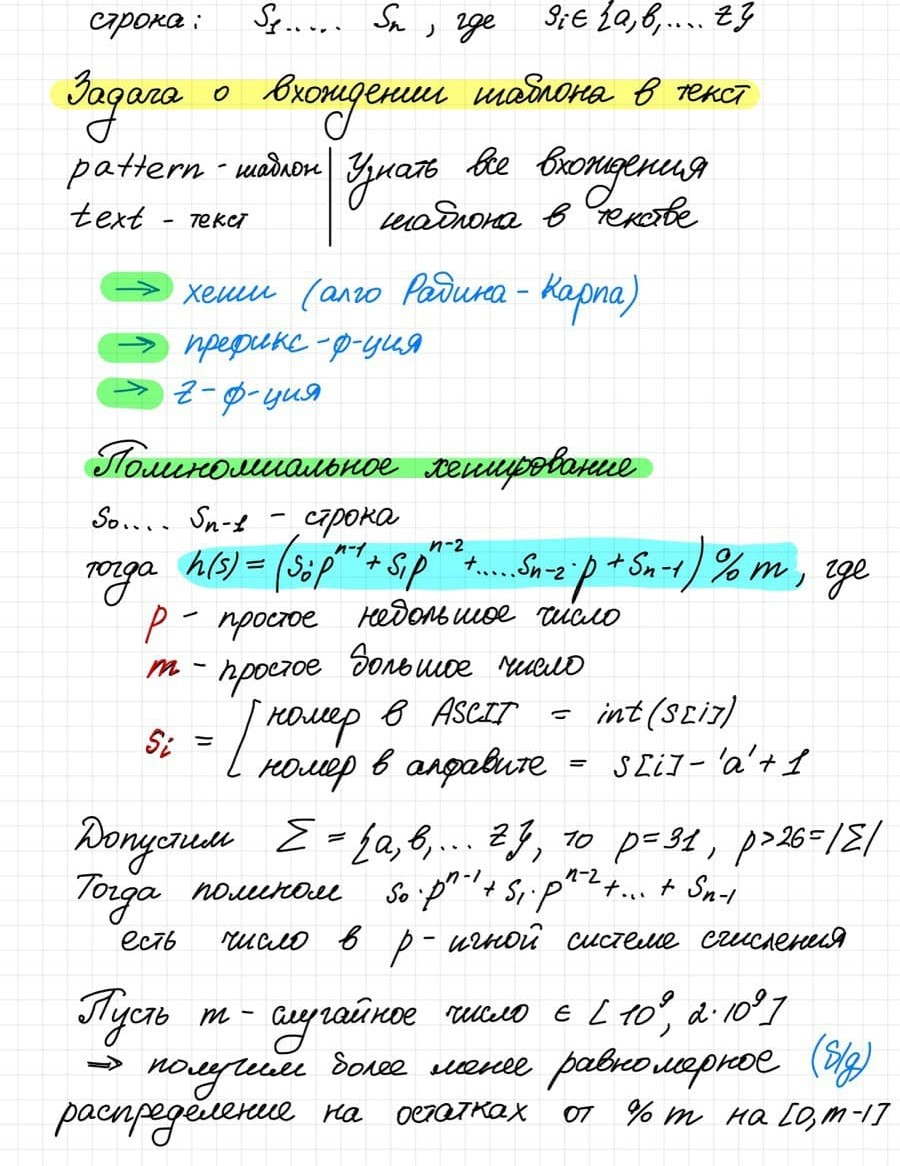
\includegraphics[width=1\linewidth]{images/hashing1.jpg}
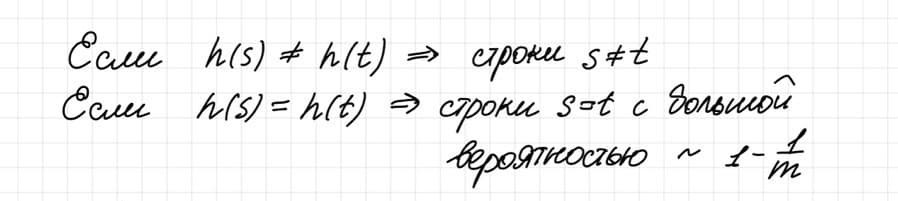
\includegraphics[width=1\linewidth]{images/hashing2.jpg}
\newpage{}

\section{Алгоритм Рабина—Карпа.}

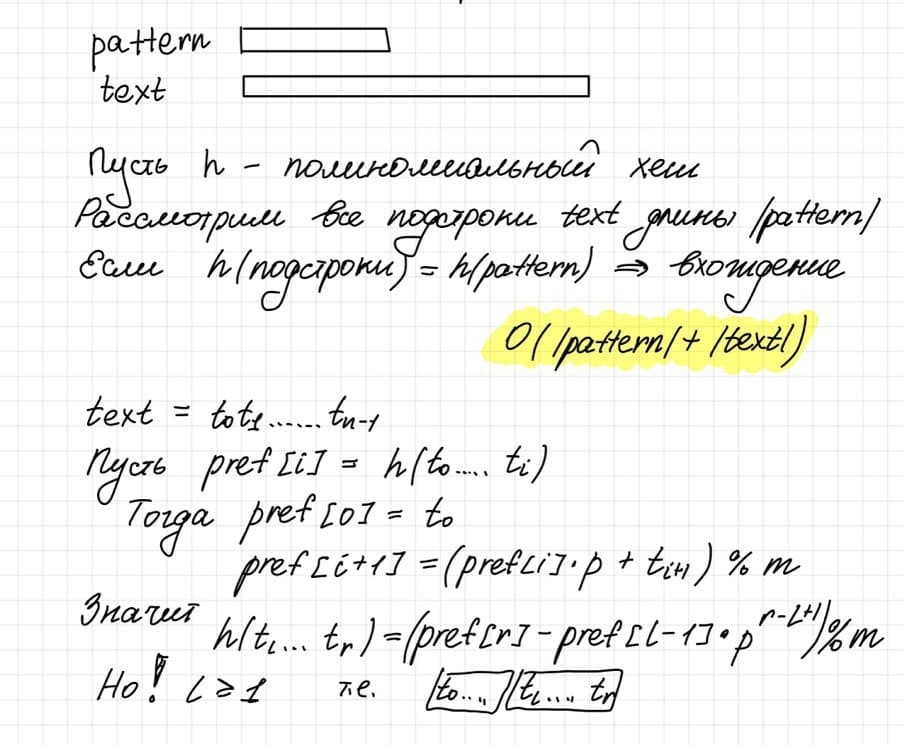
\includegraphics[width=1\linewidth]{images/Rabin-Carp.jpg}
\newpage{}

\section{Префикс-функция: определение, алгоритм нахождения за O(|s|) и применение для нахождения вхождений шаблона в текст.}
\subsection{3. Свойства класса автоматных языков. Замкнутость относительно булевых операций.}

\Def Полный ДКА.
Полный ДКА (ПДКА) - ДКА, для которого выполнено:
$$\forall a \in \Sigma, q \in Q \,\,\, |\Delta (q, a)| = 1$$

\Statement Для любого автоматного языка $L$ существует ПДКА $M$, такой что $L(M) = M$ (т.е. автоматы распознают одинаковое множество слов);

Метод построения ПДКА из ДКА:\\
1) строим ''стоковую'' вершину.\\
2) Добавляем из всех вершин переходы по недостающим буквам в "сток".

\begin{figure}[h]
    \hspace{-4ex} \begin{minipage}[h]{1\linewidth}
    \center{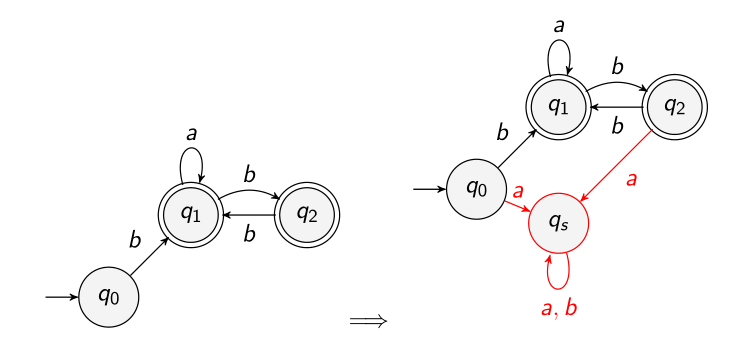
\includegraphics[width=0.6\linewidth]{1_3_1.png}}
    \end{minipage}
    \hspace{-4ex}
\end{figure}

Появятся ли новые слова? - нет, потому что, если мы попали в стоковую вершину, то не сможем ''выбраться'' из неё.

\Def Итерация Клини для языка L.
$$L^* = \cup_{k = 0}^{\infty}L^k$$

\Th Класс автоматных языков замкнут относительно\\
1. Конкатенации\\
2. Объединения\\
3. Пересечения\\
4. Итерации Клини\\
5. Дополнения

\Proof
Далее будем рассматривать только НКА с одним завершающим состоянием.
Для того чтобы после операции у итогового автомата было одно завершающее состояние, добавляем состояние и соединяем завершающие состояния с ним с помощью $\varepsilon$-переходов. (делаем новое состояние - завершающим, а старые - не завершающими)

1) Конкатенация $M_1$ и $M_2$:

Соединяем $\varepsilon$-переходами завершающее состояние $M_1$ со стартовыми состояниями $M_2$.
\begin{center}
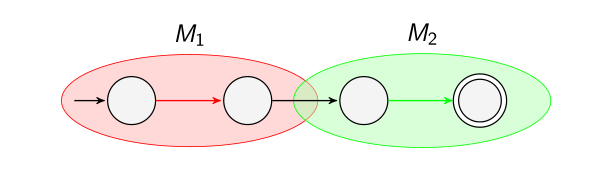
\includegraphics[width=0.45\linewidth]{1_3_2.png}
\end{center}

2) Объединение $M_1$ и $M_2$:

Добавляем стартовое состояние. Соединяем её со стартовыми состояниями $M_1$ и $M_2$ с помощью $\varepsilon$-переходов. 
\begin{center}
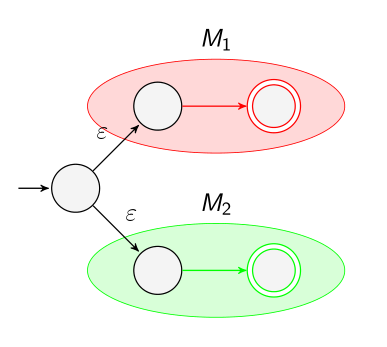
\includegraphics[width=0.25\linewidth]{1_3_3.png}
\end{center}

4) Итерации Клини над $M_1$:

Добавляем стартово-завершающее состояние. С помощью $\varepsilon$-переходов соединяем её с начальными состояниями $M_1$, а завершающее состояния $M_1$ с ней.
\begin{center}
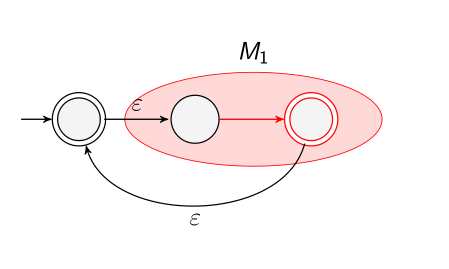
\includegraphics[width=0.32\linewidth]{1_3_4.png}
\end{center}

3) Пересечение $M_1$, $M_2$:

Строим "декартово произведение" автоматов с одно буквенными переходами.

\begin{center}
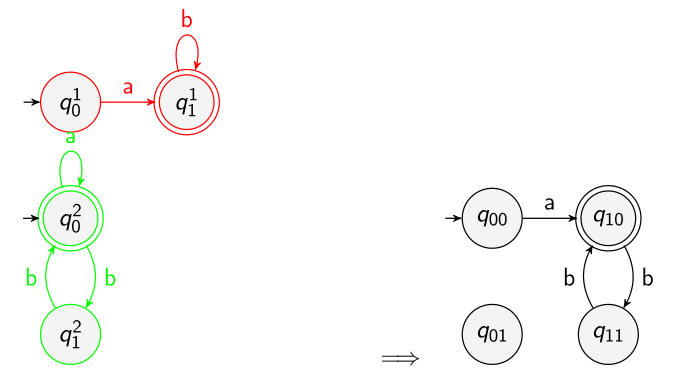
\includegraphics[width=0.55\linewidth]{1_3_5.png}
\end{center}

То есть пересечение будет состоять из состояний, каждому из которых соответствует пара чисел $(i, j)$, это номера состояний из $M_1$ и $M_2$ соответственно, которым это состояние соответствует. И между состояниями $(i_1, j_1)$ и $(i_2, j_2)$ будет проходить ребро с символом $k$, если между $i_1$ и $i_2$ проходило ребро с символом $k$ в $M_1$ и между $j_1$ и $j_2$ проходило ребро с символом $k$ в $M_2$. $(i, j)$ - стартовое состояние, если $i$ - стартовое в $M_1$, $j$ - стартовое в $M_2$. Аналогично с завершающем состоянием. 

5) Дополнение: строим ПДКА и инвертируем терминальность всех состояний.

\newpage{}

\section{z-функция: определение, алгоритм нахождения за O(|s|) и применение для нахождения вхождений шаблона в текст.}
\subsection{4. Регулярные выражения. Теорема Клини о совпадении классов регулярных и автоматных языков. Регулярный автомат, алгоритм построения.}

\Vars \\
Regex (регулярное выражение) обозначим за $R$, \newline Language (язык) -- за $L$, \newline $L(R_i)$ (язык, который задается регулярным выражением $R$) -- $L_i$.

\Def Рекурсивное определение регулярного выражения.

% \begin{minipage}[r]{0.1\linewidth} 
% %\begin{flushright}
%     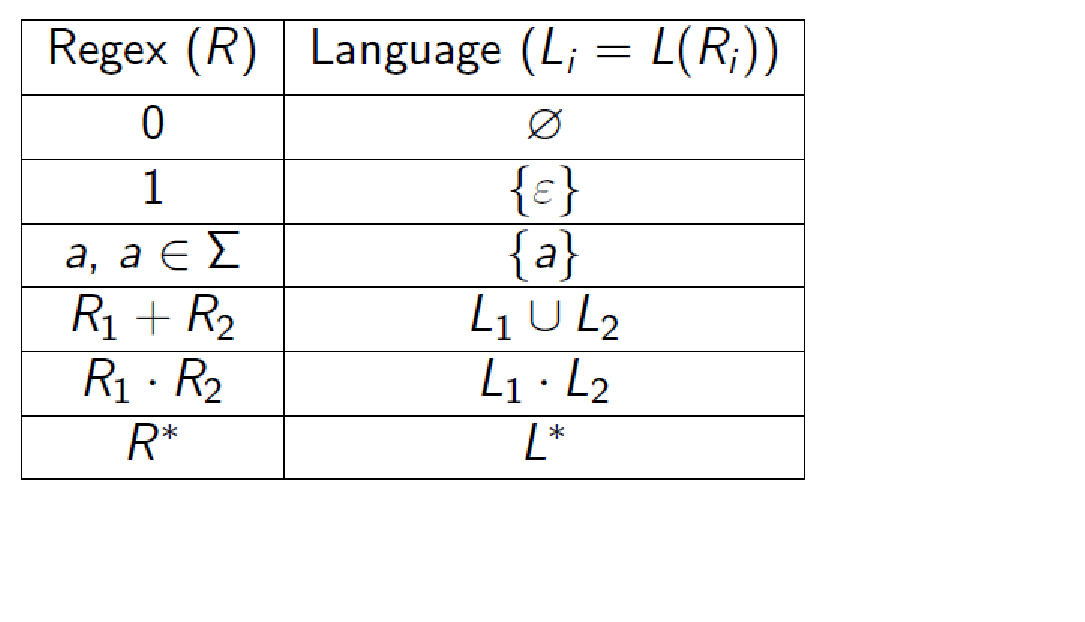
\includegraphics[width=5\linewidth]{images/1_4_1.png}
% %\end{flushright} 
% \end{minipage} 
\begin{center}
    \begin{tabular}{|c|c|}
        \hline
        $Regex (R)$ & $Language (L_i = L(R_i))$ \\
        \hline
        $0$ & $\varnothing$ \\
        $1$ & $\{ \varepsilon \}$ \\
        $a$, $a \in \Sigma$ & $\{ a \}$ \\
        $R_1 + R_2$ & $L_1 \cup L_2$ \\
        $R_1 \cdot R_2$ & $L_1 \cdot L_2$ \\
        $R^*$ & $L^*$ \\
        \hline
    \end{tabular}
\end{center}

Здесь $\varepsilon$ -- пустое слово, <<$\cdot$>> -- операция конкатенации языков (в полученном языке $L_1 \cdot L_2$ лежат слова вида $a_1a_2$, где слово $a_1$ лежит в языке $L_1$, а слово $a_2$ лежит в языке $L_2$), <<$*$>> -- звезда Клини.

Напомним определение звезды Клини: $V^* = \bigcup_{i=0}^{\infty} V^i$ 

\textbf{Приоритет операций} в регулярных выражениях (левее — приоритетнее): $* \rightarrow \cdot \rightarrow +$

\Def Язык $L$ -- регулярный, если он задается регулярным выражением.

\hspace{4ex}

\textbf{Теорема Клини:} Классы регулярных и автоматных языков совпадают.

\Proof Докажем два вложения:

\textbf{1. Регулярные $\subseteq$ Автоматные}

% \begin{figure}[h]
%     \begin{minipage}[h]{0.6\linewidth}
%     Индукция по построению выражения. 
    
%     Немного изменим утверждение -- докажем, что по регулярному выражению можно построить НКА с $1$ завершающим состоянием, который задает тот же язык.\\
    
%     \textit{База}: Построим автоматы для регулярных выражений: 0, 1, a.
%     \end{minipage}
%     \hspace{-4ex} \begin{minipage}[h]{0.5\linewidth}
%     \center{\includegraphics[width=0.6\linewidth]{images/4_base.jpg}}
%     \end{minipage}
% \end{figure}
% Регулярное выражение <<$0$>> -- автомат без завершающих состояний.

% Регулярное выражение <<$1$>> -- в автомате, состоящем из одной вершины, стартовая вершина помечается завершающим состоянием.

% Регулярное выражение <<$a$>> -- в автомате две вершины. Вершина номер $0$ стартовая, вершину номер $1$ помечаем как терминальную. Проводим ребро из $0$ в $1$, на котором пишем букву a.

Индукция по построению выражения. Немного изменим утверждение -- докажем, что по регулярному выражению можно построить НКА с $1$ завершающим состоянием, который задает тот же язык.

\textit{База}: Построим автоматы для регулярных выражений: $0, 1, a \in \Sigma$.
% %картинка%
\begin{figure}[h!]
    \centering
    \includegraphics[scale=0.27]{4_base.jpg}
\end{figure}
% \newline \center{\includegraphics[width=0.29\linewidth]{4_base.jpg}}
% \begin{minipage}[r]{1\linewidth} 
% %\begin{flushright}
%     % 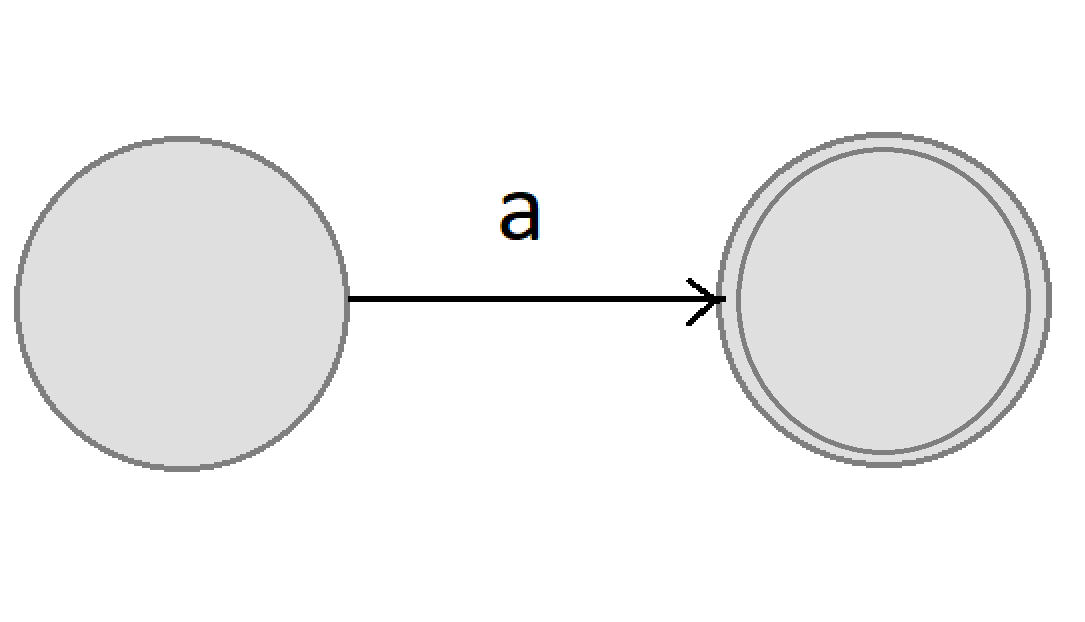
\includegraphics[width=2\linewidth]{images/1_4_2.png}
%     \center{\includegraphics[width=1\linewidth]{images/4_base.jpg}}
% %\end{flushright} 
% \end{minipage} 

\textit{Переход:}

1) $R = R_1 + R_2$. Построим автомат $A_1$ для $R_1$, для которого вершина $S_1$ -- стартовая, а вершина $F_1$ -- единственная терминальная. Для $R_2$ это будут автомат $A_2$ со стартовой вершиной $S_2$ и терминальной $F_2$.
Создадим новую вершину $S$, которая и будет стартовой в новом автомате. Из нее проведем два ребра с $\varepsilon$-переходами в $S_1$ и в $S_2$. Аналогично соединим завершающие в автоматах с новой завершающей вершиной $F$. Нетрудно доказать, что такой автомат задаст тот же язык, что и наше регулярное выражение.

2) $R = R_1 \cdot R_2$. Аналогично прошлому пункту получим автоматы для $R_1$ и $R_2$ с теми же обозначениями. Вершина $S_1$ будет стартовой в нашем новом автомате. Добавим также $\varepsilon$-переход из $F_1$ в $S_2$, уберем терминальность $F_1$.

3) $R = R_1^*$. Построим автомат $A_1$ для $R_1$ со стартовой вершиной $S_1$ и терминальной вершиной $F_1$. Создадим вершину $S$ -- новую стартовую вершину, пометим ее терминальной. Добавим из нее и из $F_1$ $\varepsilon$-переход в $S_1$.

\textbf{2. Автоматные $\subseteq$ Регулярные}

\Note{Регулярный автомат -- НКА, в котором на ребрах записаны регулярные выражения. Докажем утверждение для регулярных автоматов.}

\Note{Всякий НКА задается регулярным автоматом с 1 завершающим состоянием.}

Индукция по $|Q|$ (количеству состояний -- вершин) в регулярном автомате.

\textit{База:}

1) $|Q| = 1$. Тогда в регулярном автомате стартовое состояние является завершающим, и можно однозначно построить регулярное выражение. Такому автомату соответсвует регулярное выражение $a^*$
\newline
\begin{minipage}[r]{0.1\linewidth} 
%\begin{flushright}
    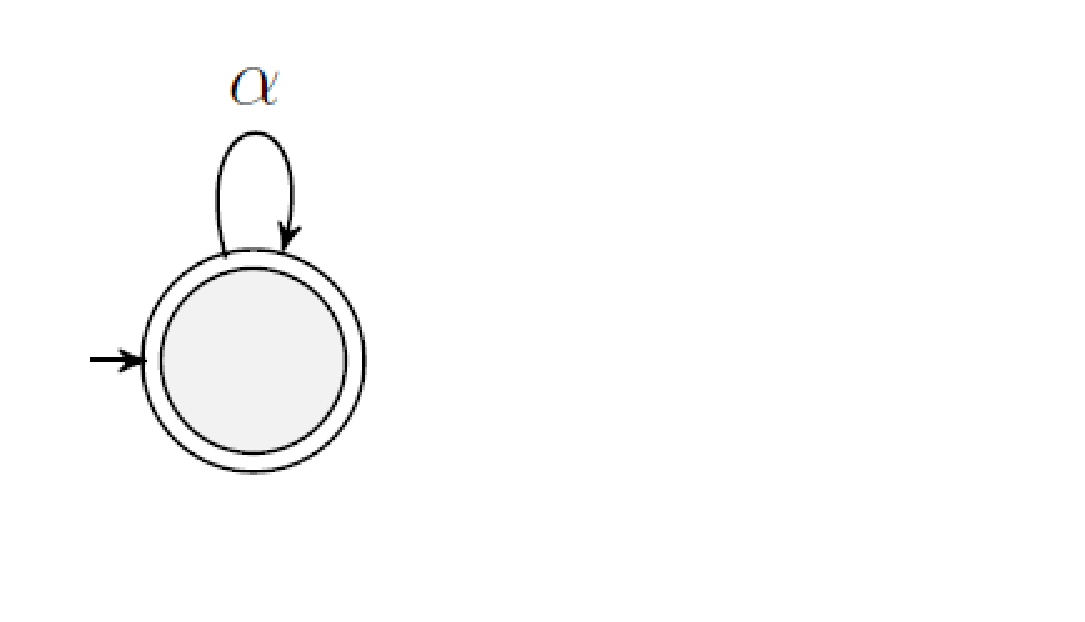
\includegraphics[width=4\linewidth]{images/1_4_3.png}
%\end{flushright} 
\end{minipage} 

2) $|Q| = 2$. Cтартовое состояние и завершающее состояние различны, и можно тоже однозначно построить регулярное выражение. Такому автомату соответсвует регулярное выражение $\alpha^*\beta(\gamma + \delta \alpha^* \beta)^*$
\newline
\begin{minipage}[r]{0.1\linewidth} 
%\begin{flushright}
    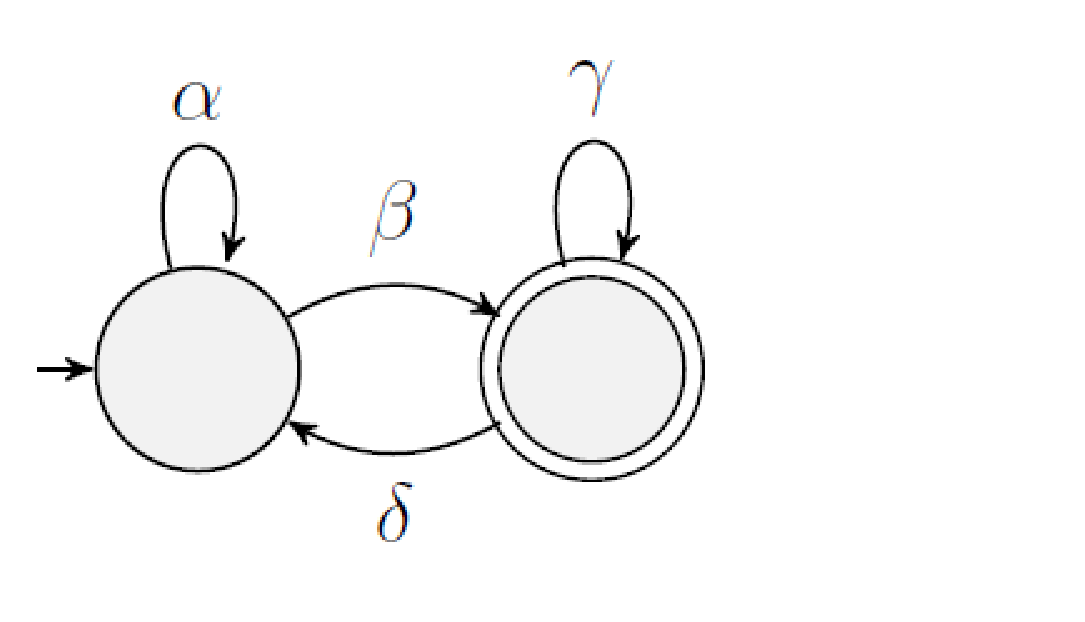
\includegraphics[width=4\linewidth]{images/1_4_4.png}
%\end{flushright} 
\end{minipage} 

Для случая, когда завершающее состояние -- это начальная вершина, регулярное выражение будет $(\gamma + \delta \alpha^* \beta)^*$.

\textit{Переход:}
\Note{Есть нестартовая и незавершающая вершина!}

1) Удаляем кратные ребра:
\begin{minipage}[r]{0.2\linewidth} 
%\begin{flushright}
    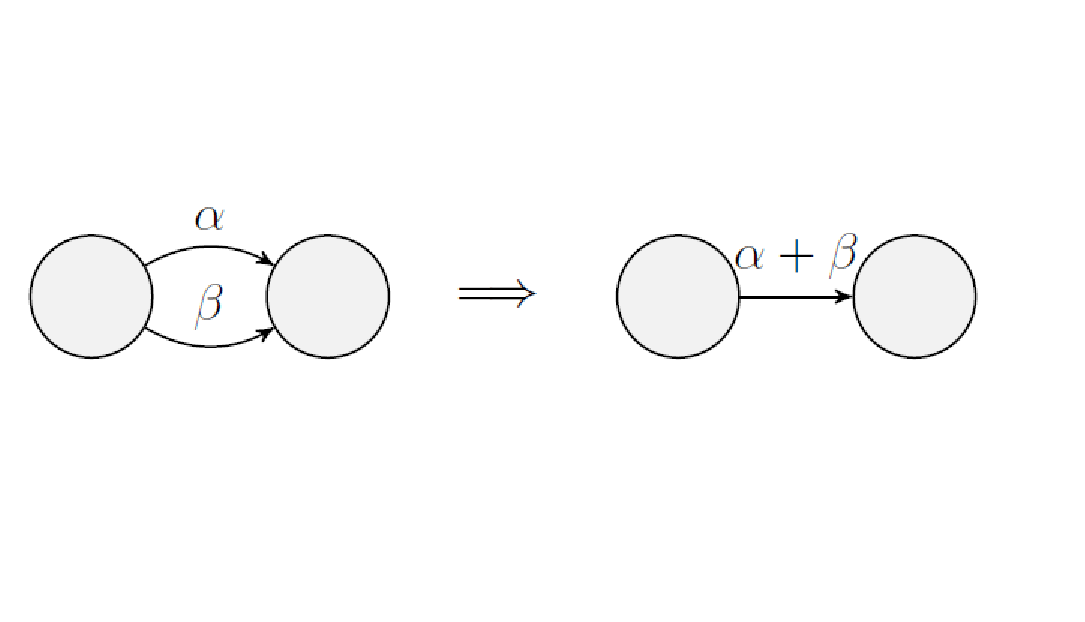
\includegraphics[width=2.5\linewidth]{images/1_4_5.png}
%\end{flushright} 
\end{minipage} 

Кратные ребра означают, что мы можем выбрать, какой символ будем использовать. Именно этот смысл и несет в себе операция <<$+$>>.

2) Добавляем циклы на себя:
\begin{minipage}[r]{0.1\linewidth} 
%\begin{flushright}
    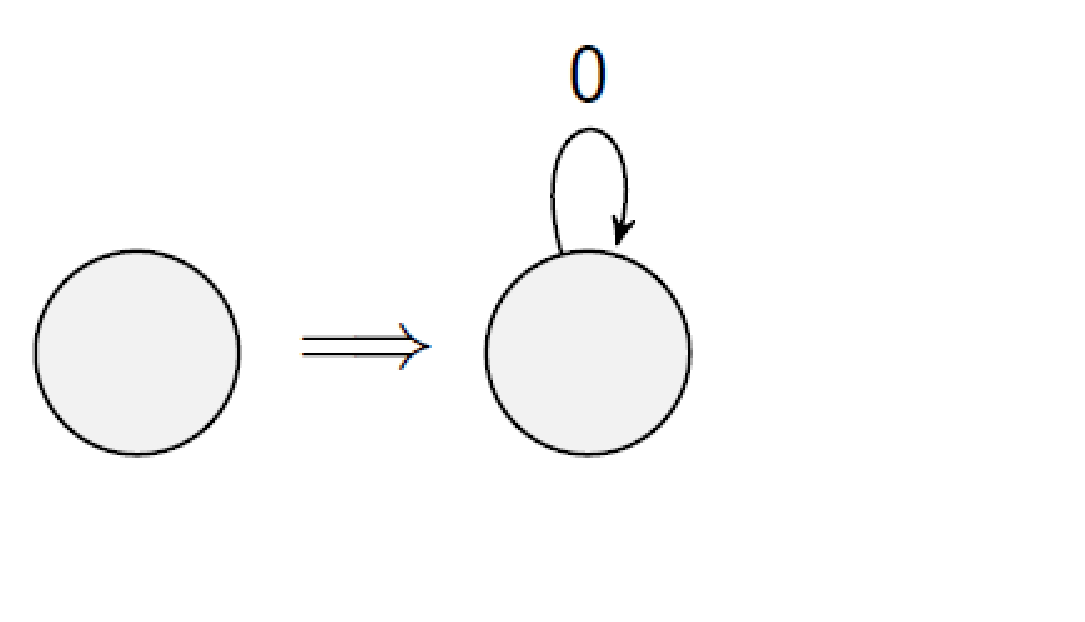
\includegraphics[width=3.5\linewidth]{images/1_4_6.png}
%\end{flushright} 
\end{minipage} 

3) Удаляем нестартовое и незавершающее состояние:

\begin{minipage}[r]{0.1\linewidth} 
%\begin{flushright}
    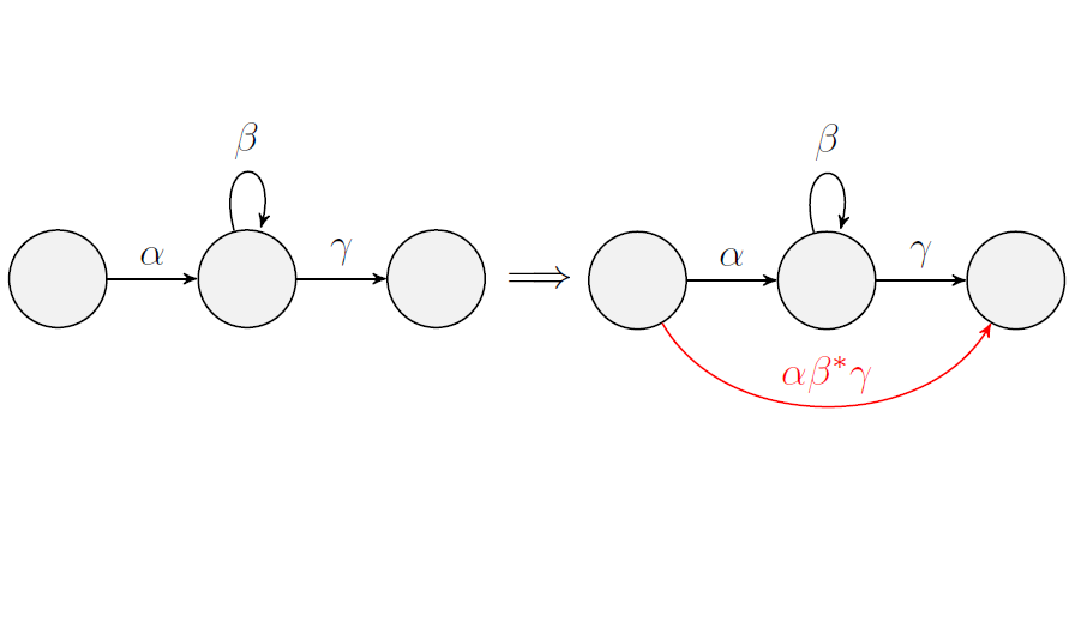
\includegraphics[width=5.5\linewidth]{images/1_4_7.png}
%\end{flushright} 
\end{minipage} 
\newline Теперь у нас на одно сотояние стало меньше, т.е. мы можем воспользоваться утверждением индукции.
\EndProof
\newpage{}

\section{Бор, построение бора по набору слов}
\section{Способы хранения бора: преимущества и недостатки.}
\section{Хранение множества слов/чисел с помощью бора. Добавление, удаление и проверка наличия.}
Бор - корневое дерево, на рёбрах которого написаны символы рассматриваемого алфавита. Если из вершины исходит несколько рёбер, то на них написаны попарно различные символы.

Бор для набора образцов ${he,she,his,hers}$:
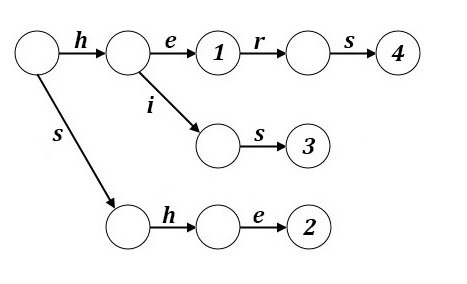
\includegraphics[width=6cm]{images/Бор.jpg}

Пусть нам дан набор слов $s_1, ..., s_n$. Построить бор для такого набора, значит, задать дерево, из корня которого по некоторому пути можно прочитать каждое из этих слов. 

Реализация: 

Построим бор по набору слов $s_1, \dots, s_n$. Для удобства заведём структуру, которая хранит вершину бора.

\begin{lstlisting}
struct node {
  map<char, int> to;
  bool term; // is node terminal? is there the final letter?
};
\end{lstlisting}

Далее заведём сам бор:

\begin{lstlisting}
vector<node> trie;
\end{lstlisting}

Реализация процедуры добаления слова в бор:

\begin{lstlisting}
void add(const string &s) {
  int v = 0;
  for (int i = 0; i < s.size(); ++i) {
    if (!trie[v].to.count(s[i])) {
      trie.push_back(node());
      trie[v].to[s[i]] = int(trie.size()) - 1;
    }
    v = trie[v].to[s[i]];
  }
  trie[v].term = true;
}
\end{lstlisting}

\Note Вместо $map$ подойдут и другие структуры. Например, можно использовать массив длины $|\Sigma|$, где несуществующие значения заполнены $-1$. Подойдёт так же и хеш-таблица.

Сравним их по памяти. Массив: $|\Sigma|$, $map$ и хеш-таблица: $k$ (число исходящих из вершины рёбер).

Сколько нужно ждать выполнения запроса? Массив: $O(1)$. $map$: $O(log k)$. Хеш-таблица: $O(1)$ в среднем.

\section{Алгоритм Ахо—Корасик: определение суффиксных ссылок (link) и переходов по буквам (to).}

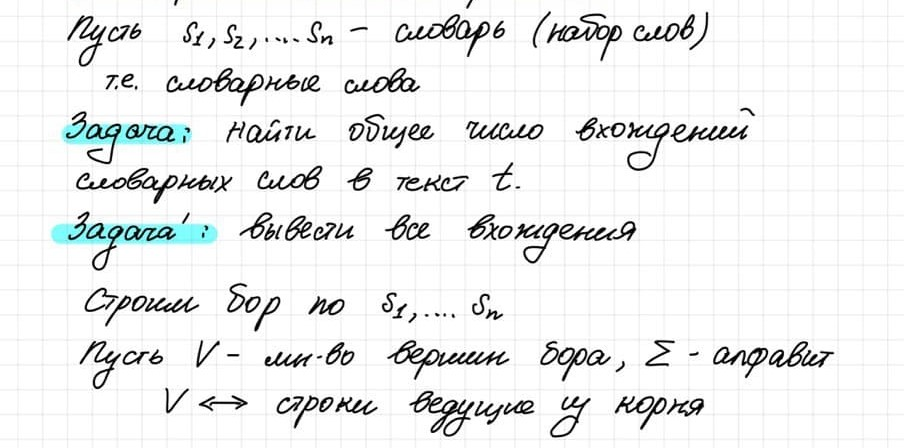
\includegraphics[width=1\linewidth]{images/Aho-Corasic1.jpg}
\newline 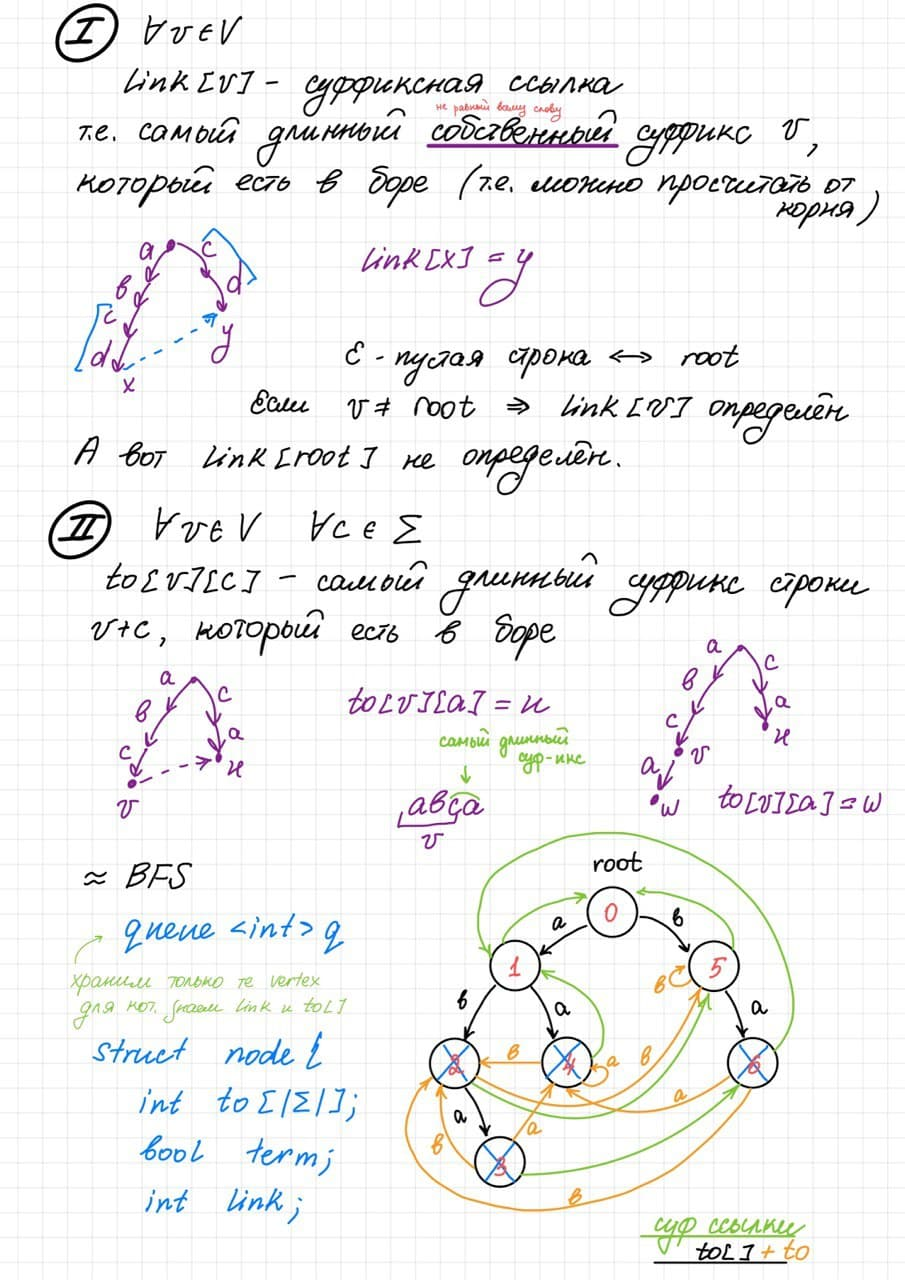
\includegraphics[width=1\linewidth]{images/Aho-Corasic2.jpg}

\section{Алгоритм Ахо—Корасик: реализация, корректность, асимптотика.}

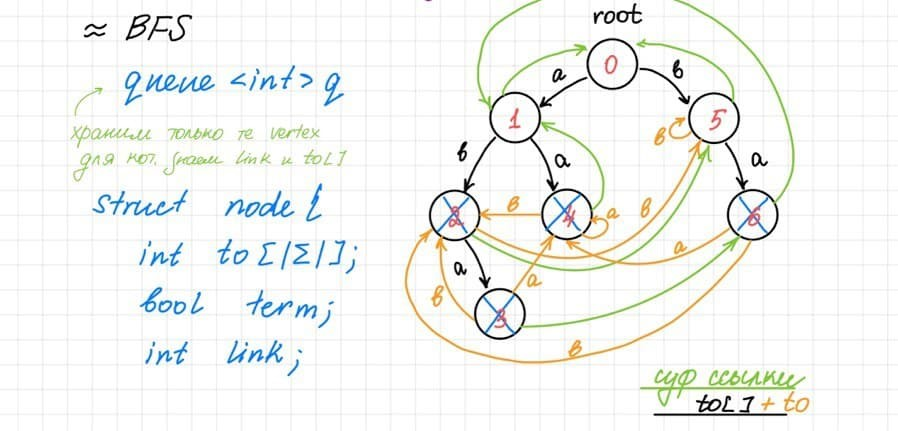
\includegraphics[width=1\linewidth]{images/Building_Aho-Corasic1.jpg}
\newline 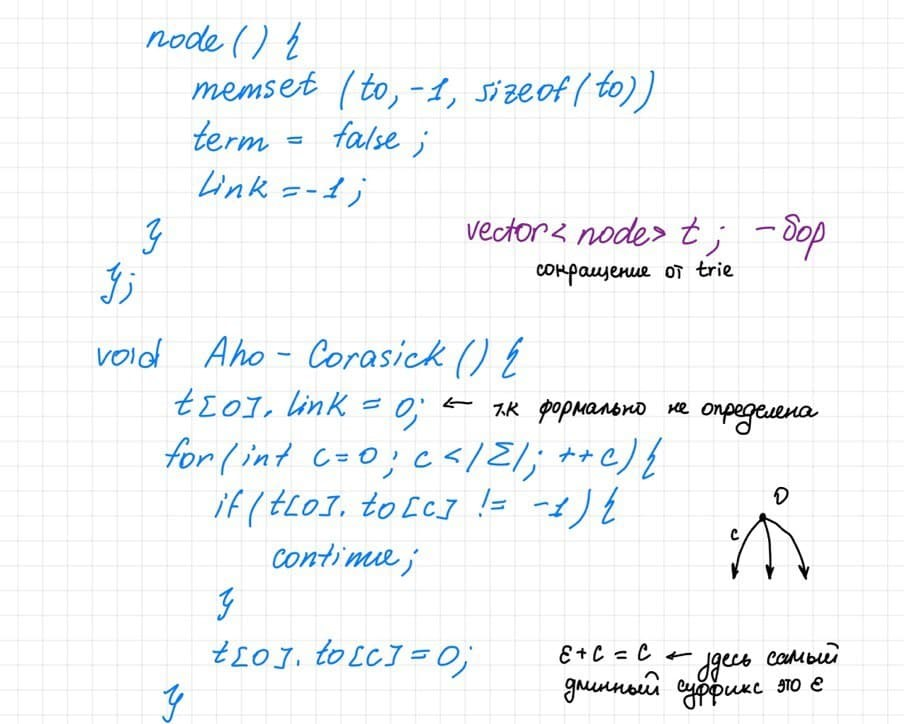
\includegraphics[width=1\linewidth]{images/Building_Aho-Corasic2.1.jpg}
\newline 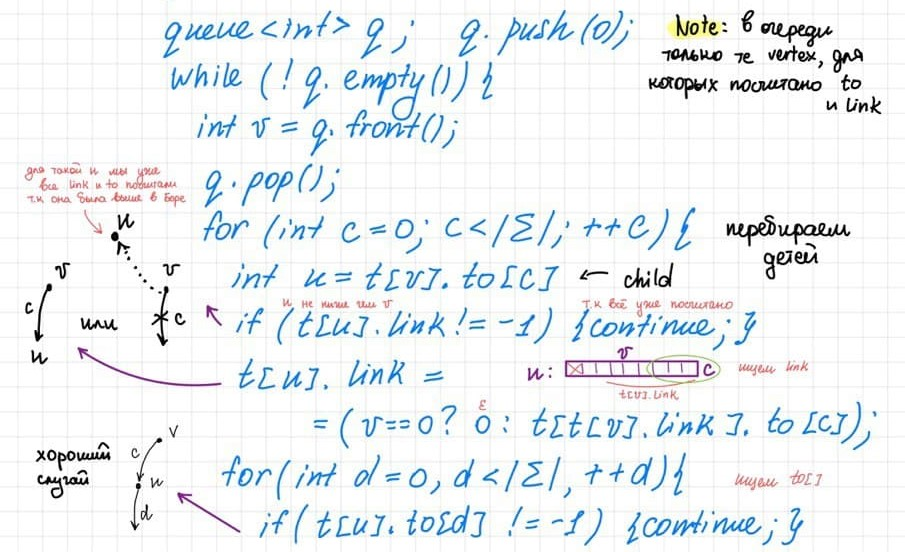
\includegraphics[width=1\linewidth]{images/Building_Aho-Corasic2.jpg}
\newline 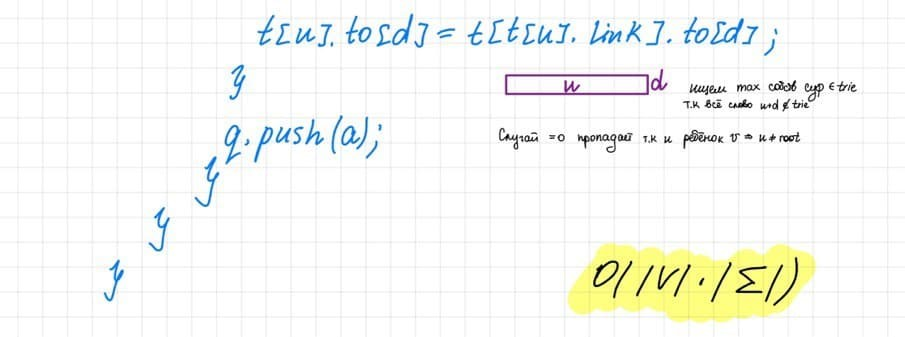
\includegraphics[width=1\linewidth]{images/Building_Aho-Corasic3.jpg}

\section{Подсчёт числа вхождений словарных слов в текст с помощью алгоритма Ахо—Корасик.}
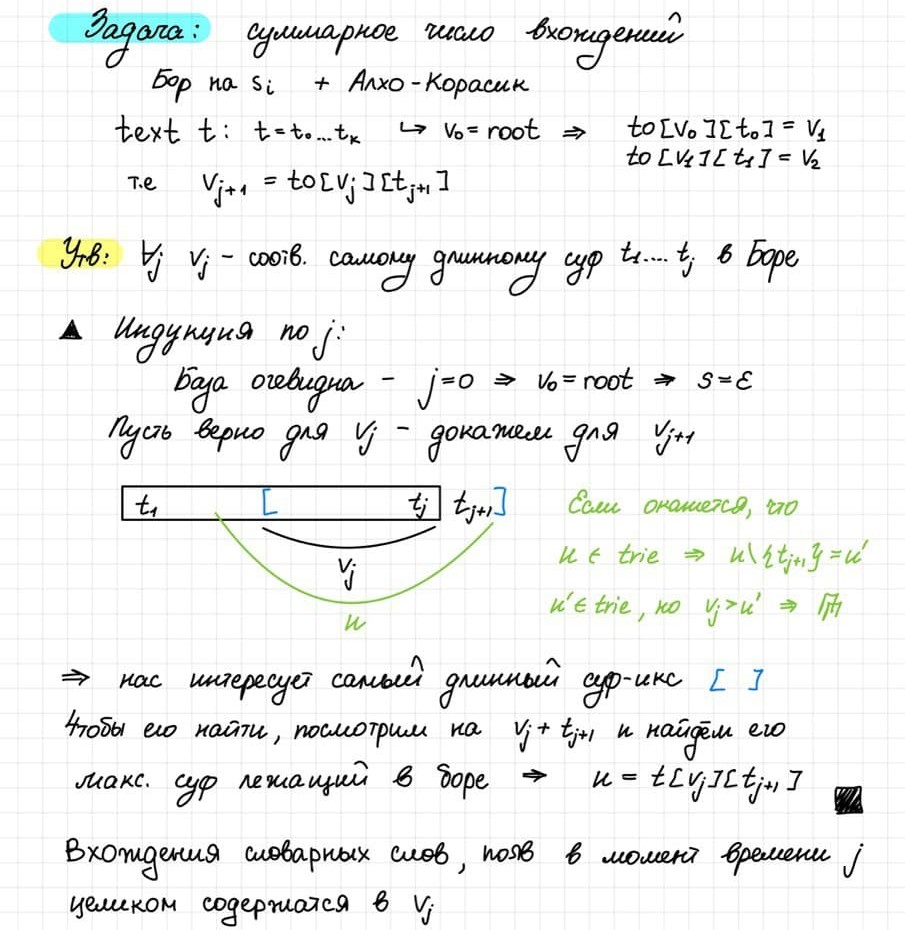
\includegraphics[width=1\linewidth]{images/Task_Aho-Corasic1.jpg}
\newline 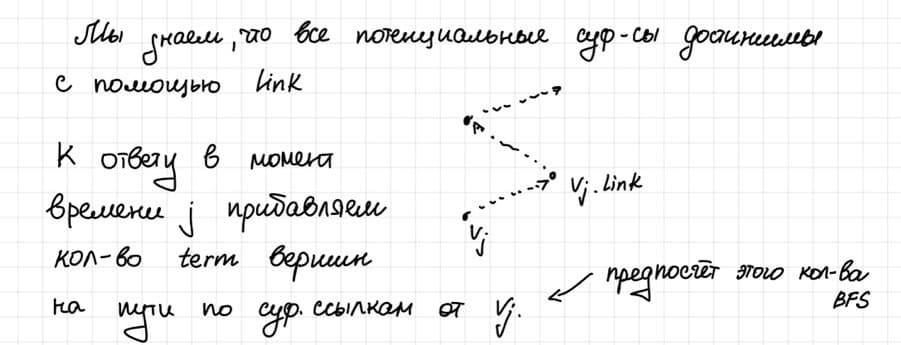
\includegraphics[width=1\linewidth]{Task_Aho-Corasic2.jpg}

\section{Определение суффиксного массива и массива lcp.}

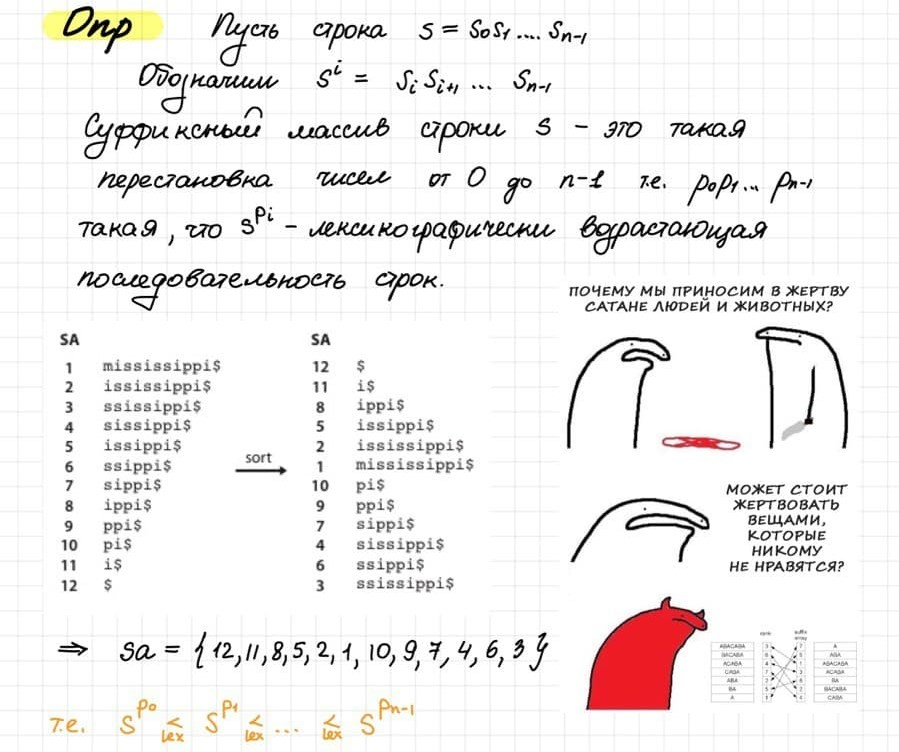
\includegraphics[width=1\linewidth]{images/SA1.jpg}
\newline 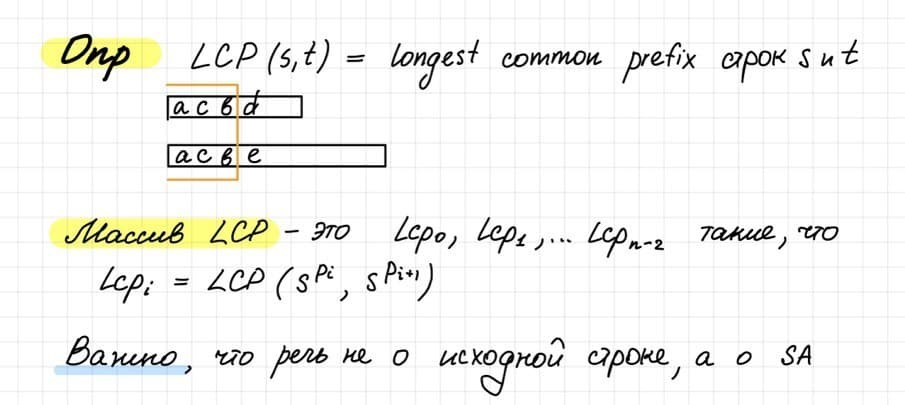
\includegraphics[width=1\linewidth]{images/SA2.jpg}
\newpage

\section{Алгоритм построения суффиксного массива строки длины $n$ за $O(n log n)$.}

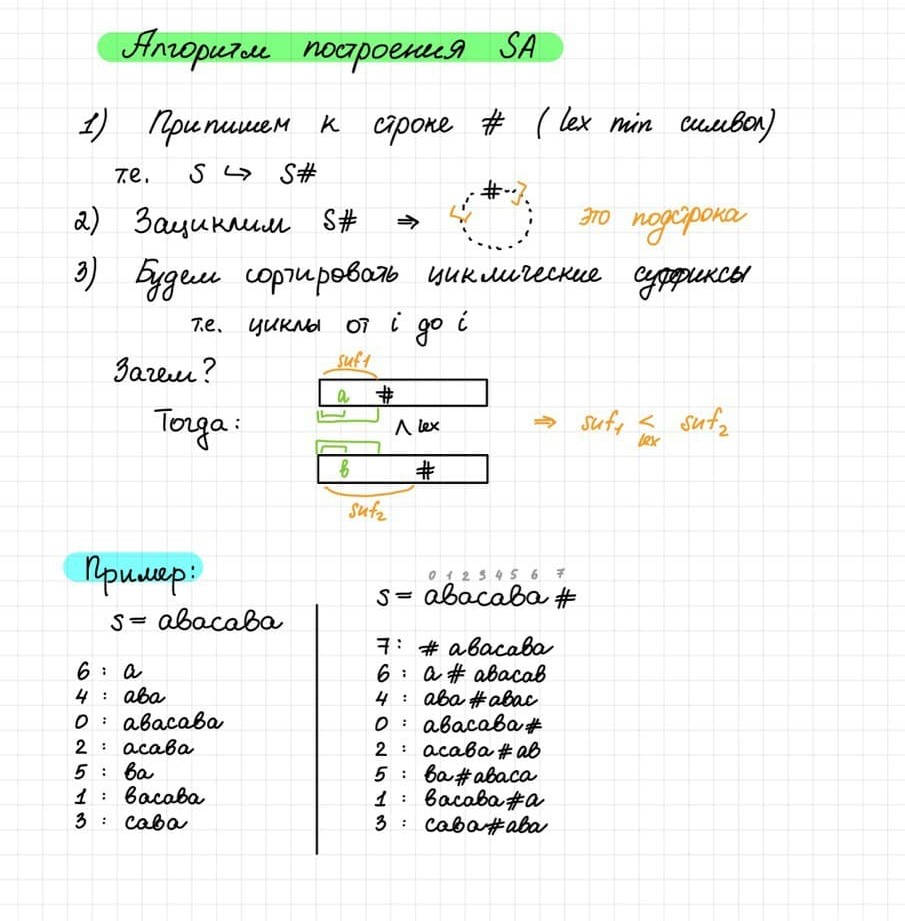
\includegraphics[width=1\linewidth]{images/Build_SA1.jpg} \newpage
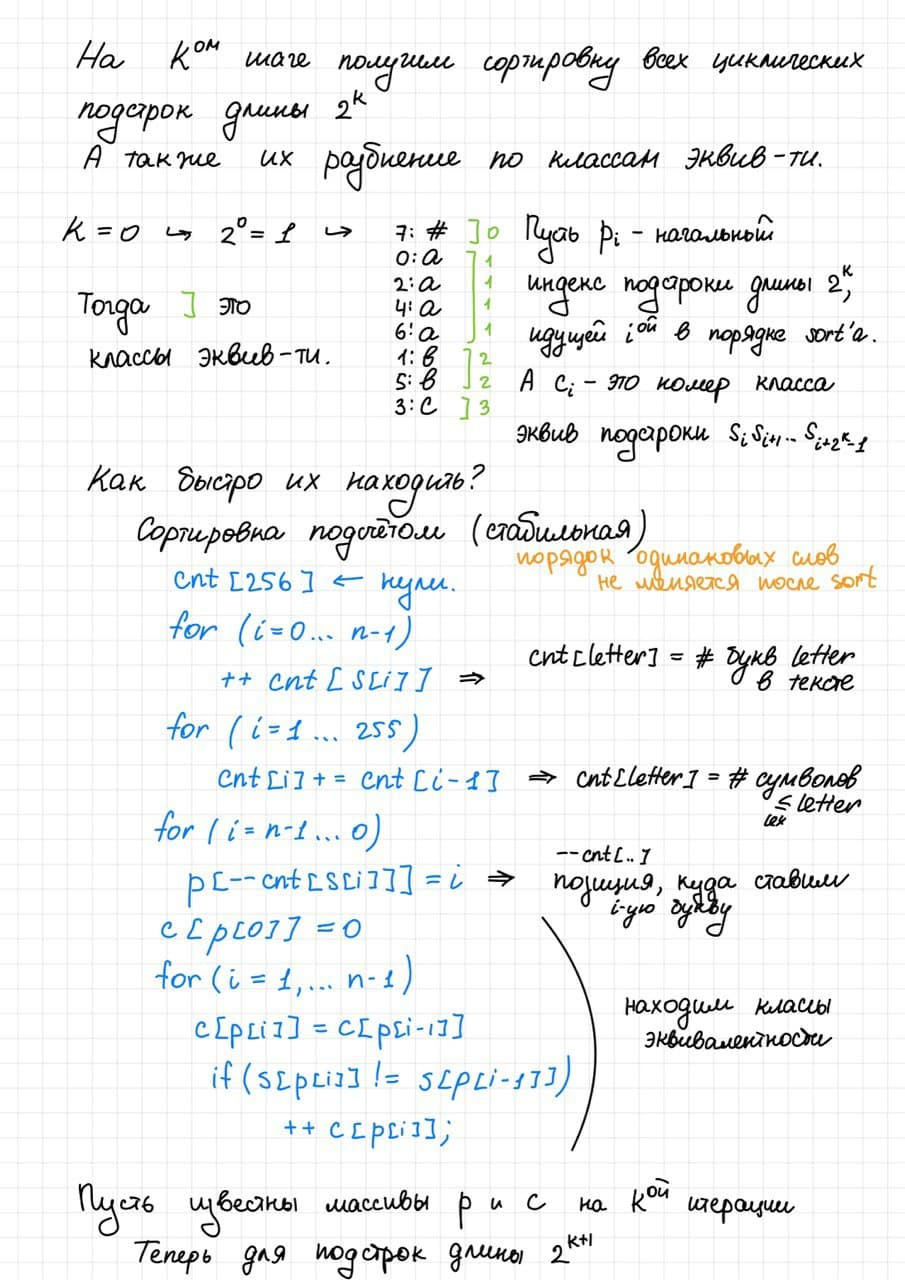
\includegraphics[width=1\linewidth]{images/Build_SA2.jpg} \newpage
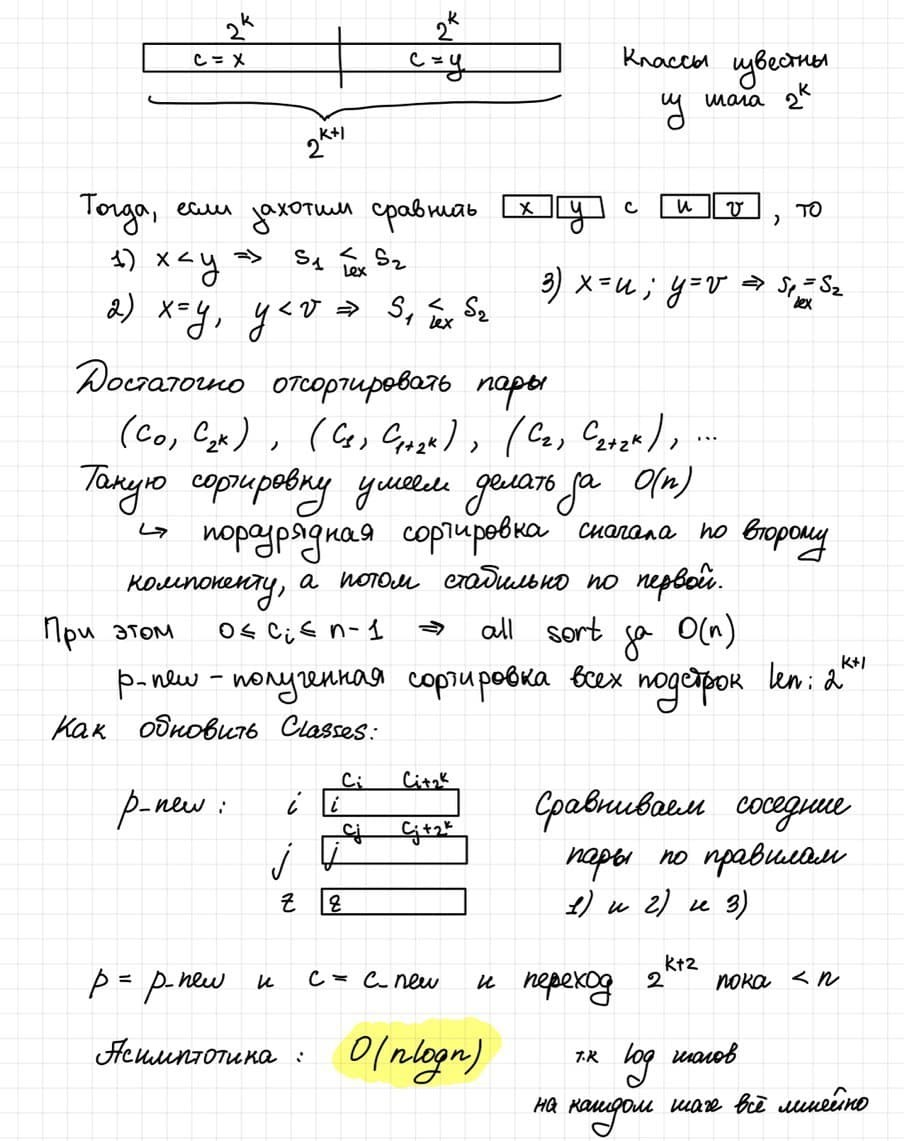
\includegraphics[width=1\linewidth]{images/Build_SA3.jpg} \newpage

\section{Алгоритм Касаи нахождения массива lcp по построенному суффиксному массиву длины $n$ за $O(n)$.}
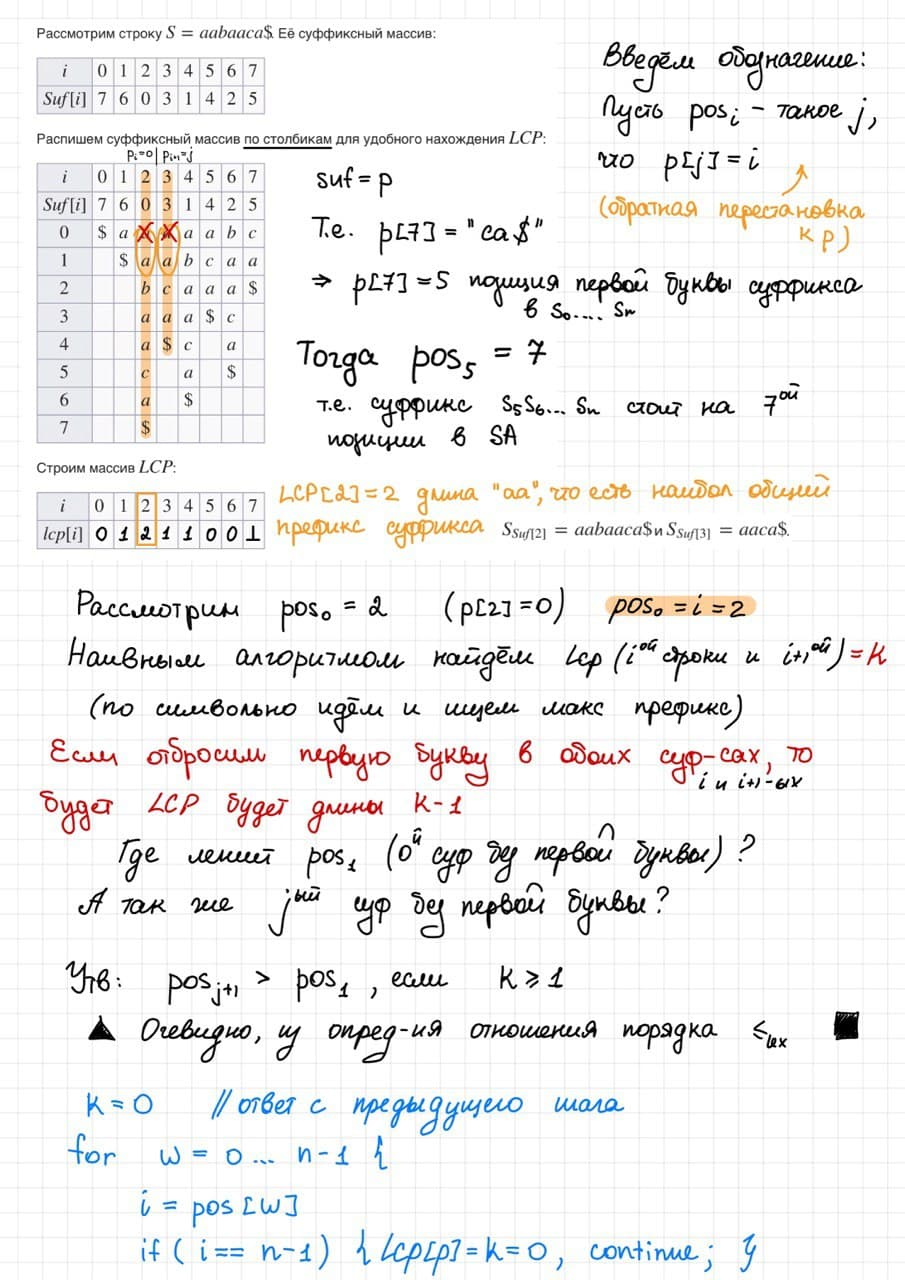
\includegraphics[width=1\linewidth]{images/Kasai1.jpg}
\newpage 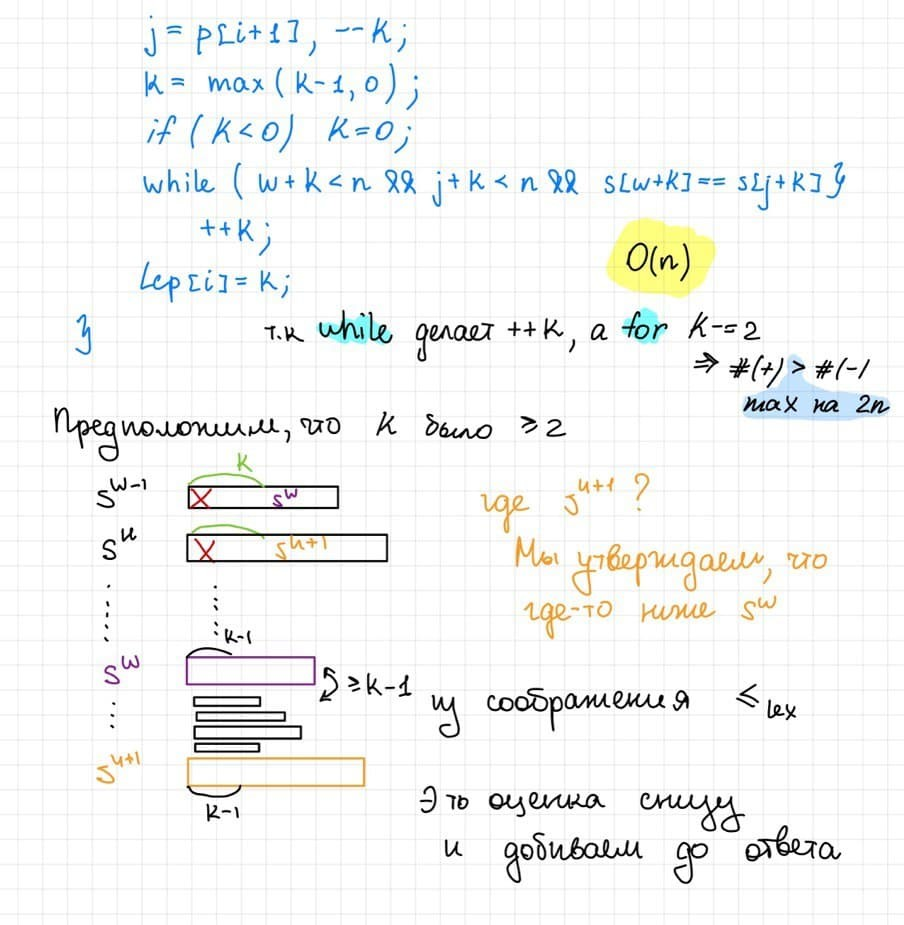
\includegraphics[width=1\linewidth]{images/Kasai2.jpg}

\section{Проверка равенства подстрок в строке: ответ на запрос за $O(1)$ с помощью sparse table и суффиксного массива.}

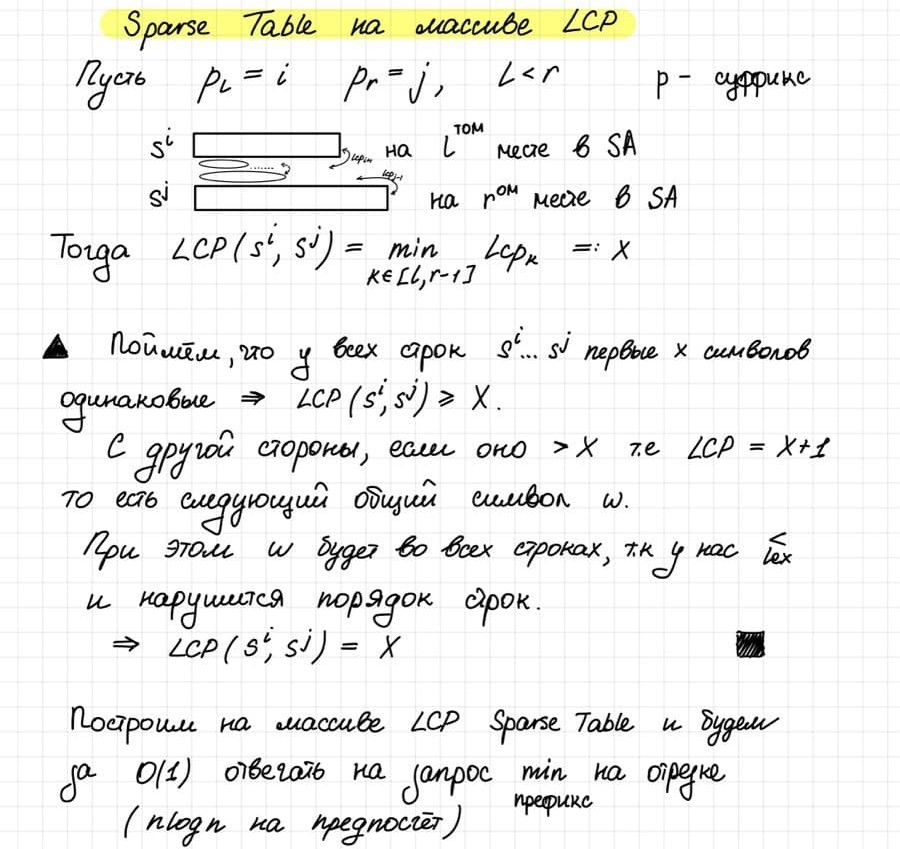
\includegraphics[width=1\linewidth]{images/Sparse_task1.jpg}
\newline 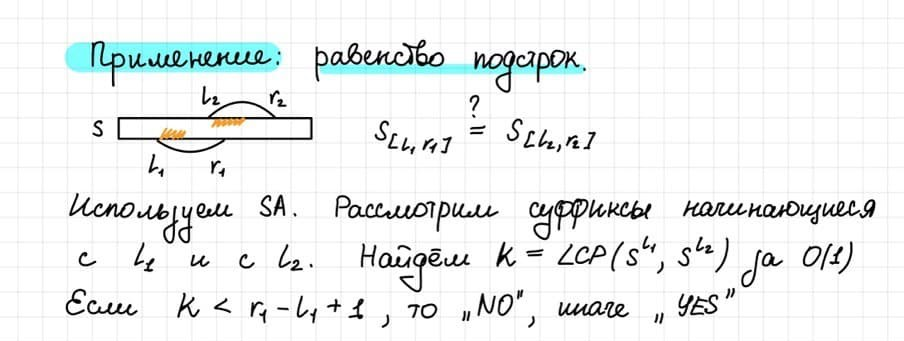
\includegraphics[width=1\linewidth]{images/Sparse_task2.jpg}
\newpage

\section{Суффиксное дерево: определение, представление в памяти, наивный алгоритм построения.}
\par \Def Сжатый бор - это бор на ребрах которого написаны подстроки данных строк, из каждой внутренней вершины которого выходят не менее 2 ребер, первые буквы которых отличаются.
\par \Def Суффиксное дерево - сжатый бор, построенный на суффиксах строки с приписанным к ней символом \$.
\par \textbf{Представление в памяти:} Для каждого ребра помимо вершины, в которую оно идет, храним индексы $l, r$ - начало и конец подстроки которая на нем написана.
\par \textbf{Наивный алгоритм построения за $O(n^2)$:} Добавляем каждый суффикс начиная с самого длинного. При добавлении нового суффикса начинаем читать его из корня. Когда не можем прочитать дальше - создаем ответвление (при необходимости создаем вершину, если ответвление должно быть на середине ребра). Отсюда так же следует, что в суффиксном дереве $O(n)$ вершин и ребер (каждый раз добавляем не больше двух вершин и не больше двух ребер).
\newpage{}

\section{Суффиксная ссылка в суффиксном дереве. Суффиксная ссылка вершины. Процедура getLink.}
\par \Def Суффиксная ссылка в суффиксном дереве - ссылка на самый длинный собственный суффикс строки соответствующей данной вершине, который есть в суффиксном дереве (то есть строка полученная отбрасыванием первого символа)
\par \Statement Суффиксная ссылка вершины - вершина
\par \Proof Вершины делятся на листовые (соответствуют суффиксам) и не листовые. Суффиксная ссылка от листовой вершины - листовая вершина или корень (так как указывает на суффикс длины на 1 меньше).
\par Рассмотрим нелистовую вершину, соответствующую строке $\alpha$. Пусть $\beta$ - строка полученная из $\alpha$ отбрасыванием первого символа, то есть на нее должна указывать суффиксная ссылка. Так как $\alpha$ не листовая в ней есть разветвление по каким-то буквам $a, b$, то есть $\alpha a, \alpha b$ - подстроки s. Так как $\beta$ - суффикс $\alpha$, то $\beta a, \beta b$ - тоже подстроки s, а значит в месте в суффиксном дереве, которое соответствует $\beta$ тоже есть разветвление, а значит это вершина \EndProof
\par \textbf{Функция getLink(pos):} Если pos - вершина, то знаем для нее суффиксную ссылку по построению дерева. Если pos - позиция на середине ребра (вершина из которой идет - v, начало - l, конец - r, отступ - k), то чтобы отбросить первой символ строки соответствующей pos можем отбросить первый символ строки соответствующей v (то есть перейти в link(v)) и оттуда прочитать k первых символов написанных на ребере, соответствующем pos.
\newpage{}

\section{Алгоритм Укконена построения суффиксного дерева.}
\par Проходим по всем символам строки и перестраиваем суффиксное дерево для каждого префикса. Пусть сейчас рассматриваем символ $c$. Разобьём все суффиксы уже рассмотренной строки на 3 класса
\begin{enumerate}
    \item Листья
    \item Не листовые вершины, из которых нет перехода по $c$
    \item Не листовые вершины из которых есть переход по $c$
\end{enumerate}
\par Покажем, что листья это несколько самых длинных суффиксов. Рассмотрим самый короткий суффикс $\beta$ являющийся листом. Из вершины соответствующей ему нет ветвления. Пусть вершина соответствующая какому-то более длинному суффиксу не листовая. Это значит, что из нее есть ветвление, то есть $\exists a, b: \alpha a, \alpha b$ - подстроки s. Но так как $\beta$ - суффикс $\alpha$, то $\beta a, \beta b$, тоже подстроки s - противоречие с тем, что в вершине, соответствующей $\beta$, нет ветвления
\par Аналогично можно показать, что третий класс - это несколько самых коротких суффиксов. Рассмотрим самый длинный суффикс $\alpha$, из которого есть переход по $c$. Рассмотрим более короткий суффикс $\beta$ - он является суффиксом $\alpha$ и если из него нет перехода по $c$, то и из $\alpha$ не должно быть (см. прошлый абзац) - противоречие.
\par Вернемся к алгоритму: нам нужно в конец каждого суффикса добавить символ $c$ и сместить терминальность вниз (показать что теперь суффиксы оканчиваются в новых вершинах)
\begin{enumerate}
    \item Листья всегда остаются листьями (мы просто дописываем каждый раз на последнее ребро $c$) $\Rightarrow$ в момент превращения суффикса в лист можно записать на нем сразу всю оставшуюся строку и забыть про него
    \item Рассмотрим 2 класс. Нам нужно добавить в этом месте переход по $c$ и сместить терминальность. Таким образом, рассматриваемый суффикс становится листом, а значит можно сразу написать на добавленное ребро оставшуюся строку. Как перебрать весь второй класс? Храним самого длинного представителя этого класса (назовем его curr) и просто проходим по суффиксным ссылкам до тех пор пока не придем в вершину, из которой есть переход по $c$.
    \item Для вершин из третьего класса нам нужно просто снести терминальность вниз по $c$-переходу.
\end{enumerate}
\begin{lstlisting}
for c in s {
    while ( из curr нет перехода по c ) {
        создаем переход из curr: [c, $]
        curr = getLink(curr);
    }
    curr = go(curr[c]) // смещаем терминальность
}
\end{lstlisting}
\par При создании новых вершин сразу вычисляем для них суффиксную ссылку (см. билет 16: поднимаемся к прошлой вершине и читаем символы на ребре). В конце проставляем терминальность - s и ее суффиксные ссылки (спускаемся до корня).
\par \textbf{Асимптотика:} Итераций while всего $O(n)$ так как каждую итерацию один суффикс перемещается в первый класс. Осталось посмотреть только на асимптотику getLink (суммарно она линейна).

\par Поймём, почему это так. Пусть $depth(v)$ — это количество рёбер от корня до $v$ (если последнее ребро не подное, то его тоже учитываем). Посмотрим, как $getLink(curr)$ влияет на $depth(curr)$. 
\begin{enumerate}
    \item Сначала $depth$ уменьшается на $1$ при (curr $\rightarrow$ p) (поднимаемся к прошлой вершине)
    \item Затем изменяем $p$ на $link(p)$; тогда глубина не может измениться меньше, чем на $-1$.
    \item В конце глубина увеличится хотя бы на 1 (читаем k символов)
\end{enumerate}  Всего getLinkов $O(n)$ - для каждого суффикса. Пусть спусков второго типа $l$. Тогда после getLink $n \leq depth' \leq depth - 2 + l$. Значит суммарно $n \leq depth - O(n) + \sum l_i$. Тогда сумма всех $l$ - это  $O(n)$. Тогда изменений глубины $O(n)$.
\par Почему второй пункт верен? Дело в том, что суффиксная ссылка для $p$ получается отбрасыванием первого символа. Посмотрим на соответствующий несжатый бор. Если на пути до $p$ хотя бы $x$ промежуточных вершин, то на пути до $link(p)$ их хотя бы $x - 1$, и между ними есть соответствие. Значит, $depth(link(p)) \geqslant depth(p) - 1$.
\par Если $|\Sigma|$ не константа, то
\begin{itemize}
    \item[-] либо $O(n|\Sigma|)$ памяти (массив)
    \item[-] либо $O(n \log |\Sigma|)$ времени (map)
    \item[-] либо хэши (вероятностно)
\end{itemize}
\newpage{}

\section{Детерминированный конечный автомат. Принимаемые слова, распознаваемый язык. Суффиксный автомат строки $s$: определение.}

\textit{Все термины давались не очень строго, видимо важно только понимание}

Детерминированный конечный автомат -- конечный ориентированный граф, над рёбрами которого написаны буквы из алфавита, при этом из одной вершины не может выходить два ребра с одинаковыми буквами. Также у ДКА необходимо зафиксировать начальное состояние и пометить некоторые вершины терминальными.

Слово принимается ДКА, если из стартовой вершины, переходя по ребрам, соотвествующим текущей букве слова, мы окажемся в терминальной вершине.

Множество слов $\mathcal{L}(A)$, состоящим из всех принимаемых автоматом $A$ слов, называется распознаваемым языком автомата $A$.

\textit{Суффиксным автоматом строки $s$} называется минимальный ДКА $A$, такой что $\mathcal{L}(A)$ -- множество всех суффиксов строки $s$, включая $\varepsilon$. Минимальность ДКА понимается как ДКА с минимальным количеством вершин.

\newpage{}

\section{Правый контекст слова относительно языка. Эквивалентность слов.}

Пусть $\mathcal{L}$ -- язык, $x, y$ -- слова.

Правым контекстом слова $x$ относительно языка $\mathcal{L}$ называется
$R_{\mathcal{L}}(x) = \{ z\ |\ xz \in \mathcal{L} \}$.

$x \sim_{\mathcal{L}} y$, если $R_{\mathcal{L}}(x) = R_{\mathcal{L}}(y)$

$\sim_{\mathcal{L}}$ является отношением эквивалентности, поэтому можно ввести $[x]_{\mathcal{L}}$ -- класс эквивалентности $x$. 

\newpage{}

\section{Утверждение об устройстве классов эквивалентности (относительно языка, состоящего из всех суффиксов $s$).}

Пусть $\mathcal{L}$ -- язык из всех суффиксов $s$, $u, v$ -- подстроки $s$.

\textbf{Утверждение 1.} Если $u \sim_{\mathcal{L}} v$, то либо $u$ -- суффикс $v$, либо $v$ -- суффикс $u$.

\underline{Доказательство}

$
    u \sim_{\mathcal{L}} v \Rightarrow \exists w\ :\ uw \in \mathcal{L},
    vw \in \mathcal{L}
$, а значит $vw$ и $uw$ являются суффиксами $s$, то есть либо
$uw$ -- суффикс $vw$ (следовательно, $u$ -- суффикс $v$), либо
$vw$ -- суффикс $uw$ (следовательно, $v$ -- суффикс $w$).

\textbf{Утверждение 2. (о структуре классов эквивалентности)} Пусть $C$ -- какой-то класс эквивалентности. Тогда $C$ -- какая строка и несколько её самых длинных суффиксов.

\underline{Доказательство}

Пусть $u$ -- самая длинная строка в $C$. Тогда остальные строки из $C$ -- её суффиксы (по утверждению 1).

Пусть $v \in C$. Тогда докажем, что все суффиксы длиннее $v$ также лежат в $C$ (это эквивалентно тому, что требуется доказать).

Так как $v \in C$, $R_{\mathcal{L}}(v) = R_{\mathcal{L}}(u)$. Пусть $w$ -- суффикс $u$, причём $|w| > |v|$.

Тогда $R_{\mathcal{L}}(w) \subset R_{\mathcal{L}}(v)$, так как $v$ -- суффикс $w$. Аналогично, $R_{\mathcal{L}}(u) \subset R_{\mathcal{L}}(w)$.

Получается, что $R_{\mathcal{L}}(u) \subset R_{\mathcal{L}}(w) \subset R_{\mathcal{L}}(v)$. Теперь, воспользовавшись тем, что $R_{\mathcal{L}}(u) = R_{\mathcal{L}}(v)$, получим, что $R_{\mathcal{L}}(w) = R_{\mathcal{L}}(u)$, то есть $w \in C$.

\newpage{}

\section{Суффиксный автомат: обозначения $[x]$, $longest(C)$, $len(C)$, $link(C)$. Формула для $|C|$.}

Пусть $s$ -- строка, $\mathcal{L}$ -- язык из всех суффиксов $s$, $C$ -- класс эквивалентности. Введём обозначения:

$[x]_s = [x]_{\mathcal{L}}$ (класс эквивалентности $x$). Если понятно, о какой строке речь, будем писать просто $[x]$.

$longest(C)$ -- самая длинная строка в классе эквивалентности $C$.

$len(C) = |longest(C)|$

$link(C)$ -- суффиксная ссылка класса $C$: $link(C) = [x]$, где $x$ -- самый длинный суффикс $longest(C)$, который не лежит в $C$.

\textbf{Замечание.} $|C| = len(C) - len(link(C))$.

\underline{Доказательство}

Пусть $w$ -- минимальный по длине суффикс в $C$. Тогда суффикс длины $|w| - 1$ лежит уже в другом классе эквивалентности $C'$. Тогда $link(C) = C', len(C') = |w| - 1$.

По утверждению из 20 билета класс эквивалентности состоит из самый длинной строки и нескольких её самых длинных суффиксов. Получается, в нем лежат суффиксы длины $len(C), len(C) - 1, \ldots, |w|$. Следовательно, 
$|C| = len(C) - |w| + 1 = len(C) - len(link(C))$.

\newpage{}

\section{Критерий того, что $u = longest([u])$.}

\textbf{Утверждение} (критерий $longest$)

Пусть $u$ -- подстрока $s$.

Тогда $u = longest([u]_s) \Leftrightarrow u \text{ -- префикс } s, 
\text{ или } \exists a \neq b\ :\ au \text{ и } bu \text{ -- подстроки } s$.

\underline{Доказательство}

$\Leftarrow$. Пусть $u \text{ -- префикс } s, 
\text{ или } \exists a \neq b\ :\ au \text{ и } bu \text{ -- подстроки } s$. Предположим, что $u \neq longest([u]_s)$.

Тогда $\exists c : c \in \Sigma, u \sim cu$.

Понятно, что $u$ не может быть префиксом $s$, так как $u$ может быть продолжено символом $c$ влево.

Из того, что $R(u) = R(cu)$ следует, что $u$ и $cu$ имеют одинаковое множество концов вхождений в $s$, то есть строку $u$ можно продлить влево только символом $c$ (а значит не существует таких различных $a$ и $b$). Противоречие.

$\Rightarrow$. Пусть $u = longest([u]_s)$. Случай, когда $u$ -- префикс, очевидный, поэтому пусть также $u$ -- не префикс $s$.

Рассмотрим все символы перед вхождениями $u$. Нужно доказать, что среди них есть хотя бы 2 разных. Если это неверно, то они равны $d$, тогда $u \sim du$, и $|du| > |longest([du])|$. Противоречие.

\newpage{}

\section{Суффиксный автомат: устройство рёбер, ведущих в вершину $v$.}

\textbf{Утверждение.}

Пусть $v$ -- вершина автомата. Рассмотрим все вершины $u_1, \ldots, u_k$, по которым можем перейти в вершину $v$ по одному переходу. Тогда:

1) Каждый из переходов  из $u_i$ в $v$ соответствует одной и той же букве;

2) $link(u_i) = u_{i + 1}$

\underline{Доказательство}

Рассмотрим $u_k$, из которой возможно перейти в $v$ по букве $c$, 
но единственный способ получить одно из слов, которым соответствует состояние $v$ -- сделать конкатенацию $u_k$ и $c$. То же и для других классов эквивалентности.

\newpage{}

\section{Алгоритм построения суффиксного автомата: характеристика новых классов при дописывании символа $c$; изменение множества рёбер при дописывании символа $c$ в трёх случаях; проставление $len$ и $link$ у всех вершин.}

Пусть для строки $S$ построен суффиксный автомат. К $S$ приписывается символ $c$, и автомат нужно перестроить. Классами эквивалентности у нас будут представители $longest$. Как меняется множество самых длинных строк в своих классах? Если $u$ было $longest$, то есть $u = longest({[u]}_S)$, то $u$ останется $longest$. Значит, могут только появиться новые самые длинные строки, и таковой будет обязательно $Sc$, $Sc = longest({[Sc]}_{Sc})$. ${[Sc]}_{Sc}$ — множество всех суффиксов $Sc$, не являющися подстроками $S$.

Пусть $T$ -- ещё одна новая самая длинная строка $longest$. Тогда до этого она не была $longest$, а теперь стала, то есть (по критерию $longest$) не была префиксом и перед всеми её вхождениями стоял одинаковый символ $x$. Тогда $T$ могла стать $longest$ только если она является суффиксом $Sc$, и при этом перед ней стоит символ $y$, не равный $x$. Единственный кандидат на роль $T$ -- самый длинный суффикс $Sc$, который является подстрокой $S$.

Обозначим за $S_0$ наибольший суффикс $Sc$, который является подстрокой $S$, при этом $link([Sc]_{Sc}) = [S_0]_{Sc}$.

После добавления $c$ большинство рёбер в старом автомате, соответствующем $S$, сохранятся. Потенциальные изменения: 

1) Рёбра в $[Sc]$ (из этого состояния рёбер точно не будет, иначе была бы более длинная строка);

2) Если $S_0$ — новый $longest$, то состояние $q$ расщепилось, могут измениться в рёбра в состояние $q$ (они могут вести в другое состояние), а также нужно понять, откуда теперь ведут рёбра из $q$.

Больше ничего не изменится, так как неучтёнными останутся рёбра между вершинами (состояниями), которые не изменились.

Теперь поймём, какие рёбра нужно провести в $[Sc]$. На них должна быть написана одна и та же буква $c$. Скажем тогда, что мы должны провести ребро из строки класса $[u]$ в класс $[Sc]$, на котором буква $c$, если $uc$ — суффикс $Sc$, и $uc$ при этом не подстрока $S$. Пусть мы хотим пойти из $[S]$, перемещаемся по суффиксным ссылкам, и так дошли до некоторой вершины $p$.

Тут есть несколько случаев:

1)  Если из корневой (стартовой) вершины нет перехода по $c$, тогда из $S$ переходим по суффиксным ссылкам по корня, $S_0 = \varepsilon$ и $c$ не встречался в $S$. Действительно, это может быть только в том случае, если $c$ -- символ, не встречавшийся ранее и в строке, и в автомате. Кроме того, ранее мы заметили, что $link([Sc]) = [S_0]$, и суффиксная ссылка новой вершины будет вести в корень;

2) Если мы по суффиксным ссылкам дошли до вершины, из которой есть переход по $c$. Пусть $p$ -- первая найденная такая вершина. Тогда утверждаем, что из $p$ по $c$ можно перейти в $q$, которому принадлежит $S_0$. Тогда $S_0 = longest(p) + c$. Если $S_0$ не было $longest$, то он станет им, и есть шанс его расщепить. Не нужно расщеплять $q$, если и только если $S_0$ была $longest (q)$, и $len(q) = len(p) + 1$. Чтобы память не росла квадратично, храним лишь длины $longest$. Тогда состояния не меняются. Обрабатывать будем просто: скажем, что $link(Sc) = q$, и на этом закончим. Вспоминаем, что нужно проводить и как: из $u$ проведём по $c$ ребро в $Sc$, если $uc$ -- не подстрока $S$, и $u$ — суффикс $S$.

3) Теперь разберём случай, когда из $p$ есть переход по $c$ в вершину $q$, но $len(q) > len(p) + 1$. Тогда состояние $q$ придётся расщепить. Тогда можно представить строку, соответствующую $q$, и её несколько длинных суффиксов по убыванию длины. $S_0$ не является самым длинным из них. Что нужно сделать? $S_0$ будет новым $longest$, и первое новое состояние $q$ будет соответствовать суффиксам, длиннее $S_0$, второе новое $clone$ — остальным суффиксам. Рёбра могли перенаправиться: либо в оставшееся $q$, либо в $clone$. Рассмотрим суффиксный путь. Для вершин, соответствующим более длинным суффиксам строки $S$, чем $p$, ничего не изменится, исходящие рёбра, ведущие в $q$, сохранятся. А вот для остальных ситуация изменится вот так:

\begin{lstlisting}
while (p != -1 && to[p][c] == q) {
    to[p][c] = clone;
    p = link[p];
}
\end{lstlisting}
    
    Что делать с рёбрами, исходящими из $q$ и $clone$? Прежде всего заметим, что $R_{Sc} (clone) = R_{Sc} (q) \sqcup \{ \varepsilon \}$. Нужно понять, как отличаются множества вхождений строк, соответствующим классам $[q]$ и $[clone]$. $longest(q)$ не будет суффиксом $Sc$, и множество вхождений $longest(q)$ в $Sc$ совпадает с множеством вхождений в $S$. А вот у $S_0$ появилось одно новое вхождение. Для $q$ $Sc$ -- не терминальная строка, для $clone$ $Sc$ -- терминальная строка. Этим и отличается $q$ от $clone$ в плане исходящих рёбер. В итоге $to[clone] = to[q]$. Теперь проставляем ссылки. $len(clone) = len(p) + 1$, $link(clone) = link(q)$, $link(q) = clone$, $link([Sc]) = clone$.
    
\newpage{}

\section{Алгоритм построения суффиксного автомата: реализация.}

\begin{lstlisting}
struct node {
    int len, link;
    std::vector<int> to;
    int last;
};

vector<node> t;

void add(char c) {
    t.push_back(node());
    curr = t.size() - 1;
    p = last;
    while (p != -1 && t[p].to[c] == -1) {
        t[p].to[c] = curr;
        p = t[p].link;
    }
    if (p == -1) {
        t[curr].link = 0;
        last = curr;
        return;
    }
    q = t[p].to[c];
    if (t[q].len == t[p].len + 1) {
        t[curr].link = q;
        last = curr;
        return;
    }
    t.push_back(node());
    clone = t.size() - 1;
    while (p != -1 && t[p].to[c] == q) {
        t[p].to[c] = clone;
        p = t[p].link;
    }
    t[clone].to = t[q].to;
    t[clone].len = t[p].len + 1;
    t[clone].link = t[q].link;
    t[q].link = clone;
    t[curr].link = clone;
    last = curr;
}

int main() {
    t.push_back(node());
    // здесь добавляем по одному символу из строки
    return 0;
}
\end{lstlisting}

\newpage{}

\section{Алгоритм построения суффиксного автомата: асимптотика.}

\textbf{Теорема (б/д).}
В суффиксном автомате, построеннм по строке длины $n$ (начиная с некоторого $n_0$), не более чем $2n - 1$ вершин и $3n - 4$ рёбер.

Получается, что асимптотика $O(n)$, если $|\Sigma| = const$, или

$O(n \cdot \log |\Sigma|)$ (используя map) или $O(n \cdot |\Sigma|)$ (используя vector), если
$|\Sigma| \neq const$.

С учётом теоремы, единственный нетривиальный момент в доказательстве асимптотике -- нужно доказать, что перенаправлений ребер (как в 3 пункте) $O(n)$.

Пусть у нас был путь из $S$ по суффиксным ссылкам длины $m$. Весь этот путь разбивается на кусочки, из которых перенаправление ребер идет в одну и ту же вершину. Эти вершины составляют путь по суффиксным ссылкам из $clone$. Пусть в каком-то блоке $k$ вершин. Тогда вершин в пути по суффиксным ссылкам из $clone$ не больше $m + 2 - k$.

\newpage{}

\section{Алгоритм Евклида: корректность, реализация, асимптотика.}
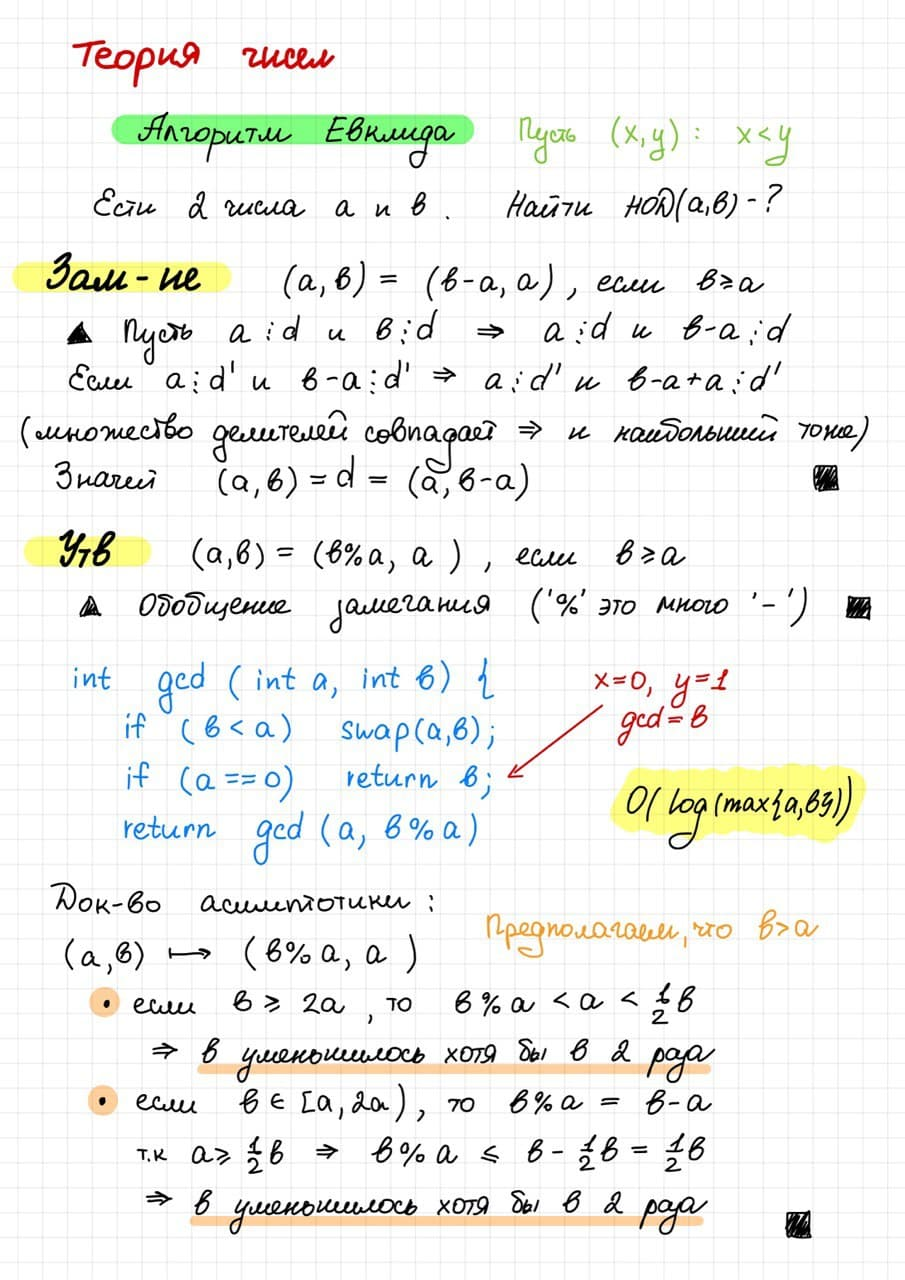
\includegraphics[width=1\linewidth]{images/Evklid.jpg}

\section{Расширенный алгоритм Евклида (нахождение решения $ax + by = (a, b)$ в целых $x, y)$.}
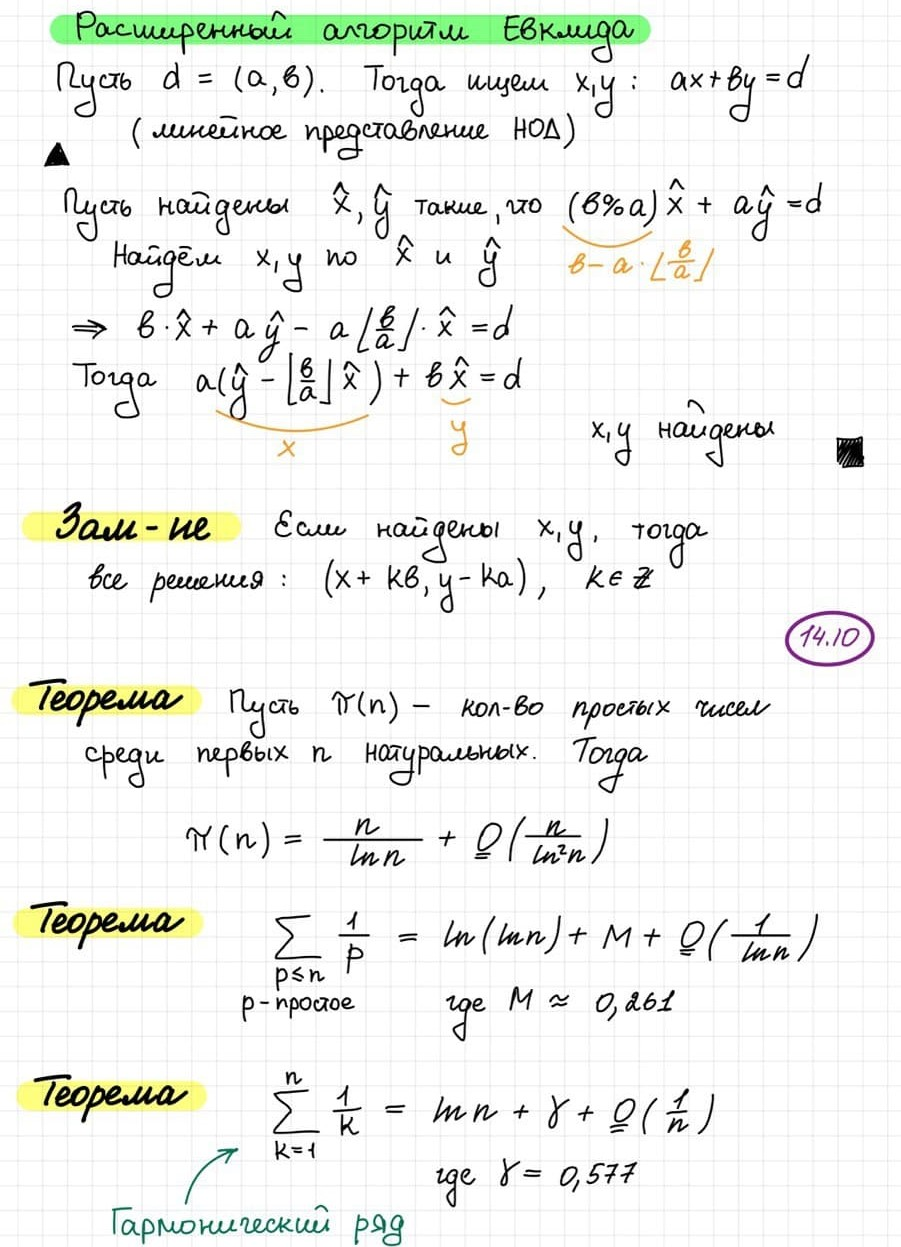
\includegraphics[width=1\linewidth]{images/Big_Evklid.jpg}

\section{Решето Эратосфена: нахождение всех простых среди $\{1, 2, \ldots, n\}$ за время $O(n\log{\log{n}})$.}
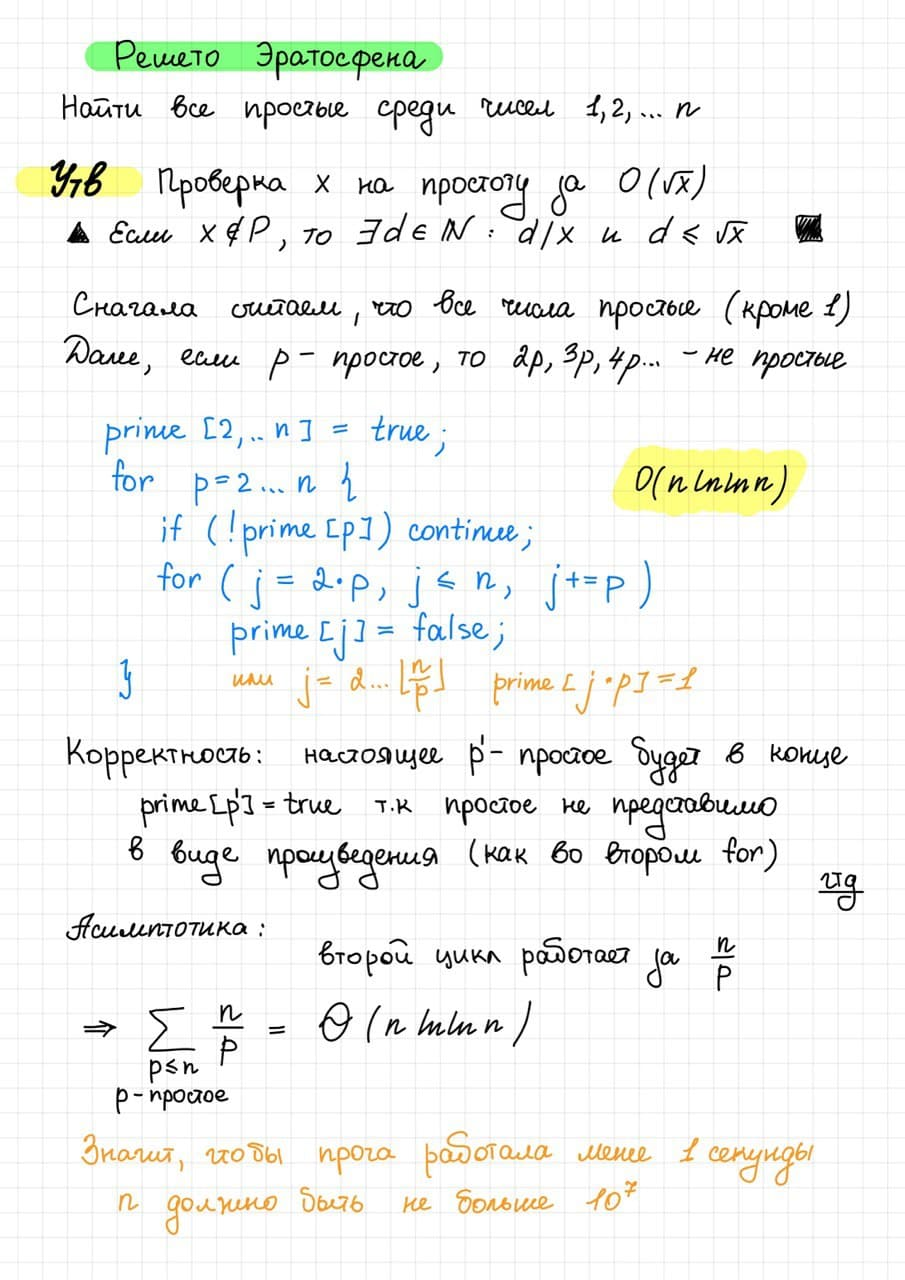
\includegraphics[width=1\linewidth]{images/Sieve.jpg}

\section{Улучшенное решето Эратосфена: нахождение минимального простого делителя для всех чисел из $\{1, 2, \ldots, n\}$.}
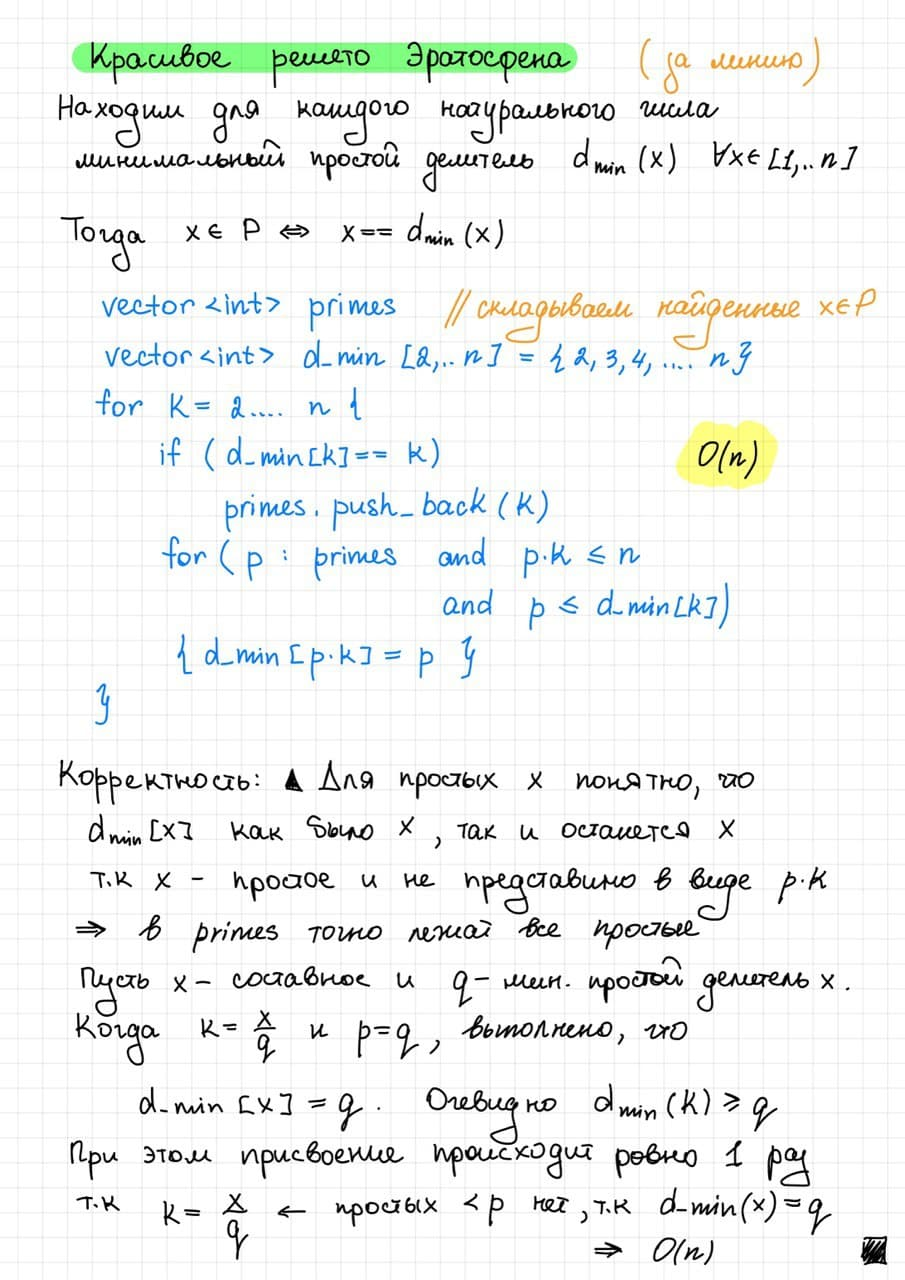
\includegraphics[width=1\linewidth]{images/Nice_sieve.jpg}

\section{Обратное к a по модулю m: достаточное условие существования, алгоритм нахождения.}
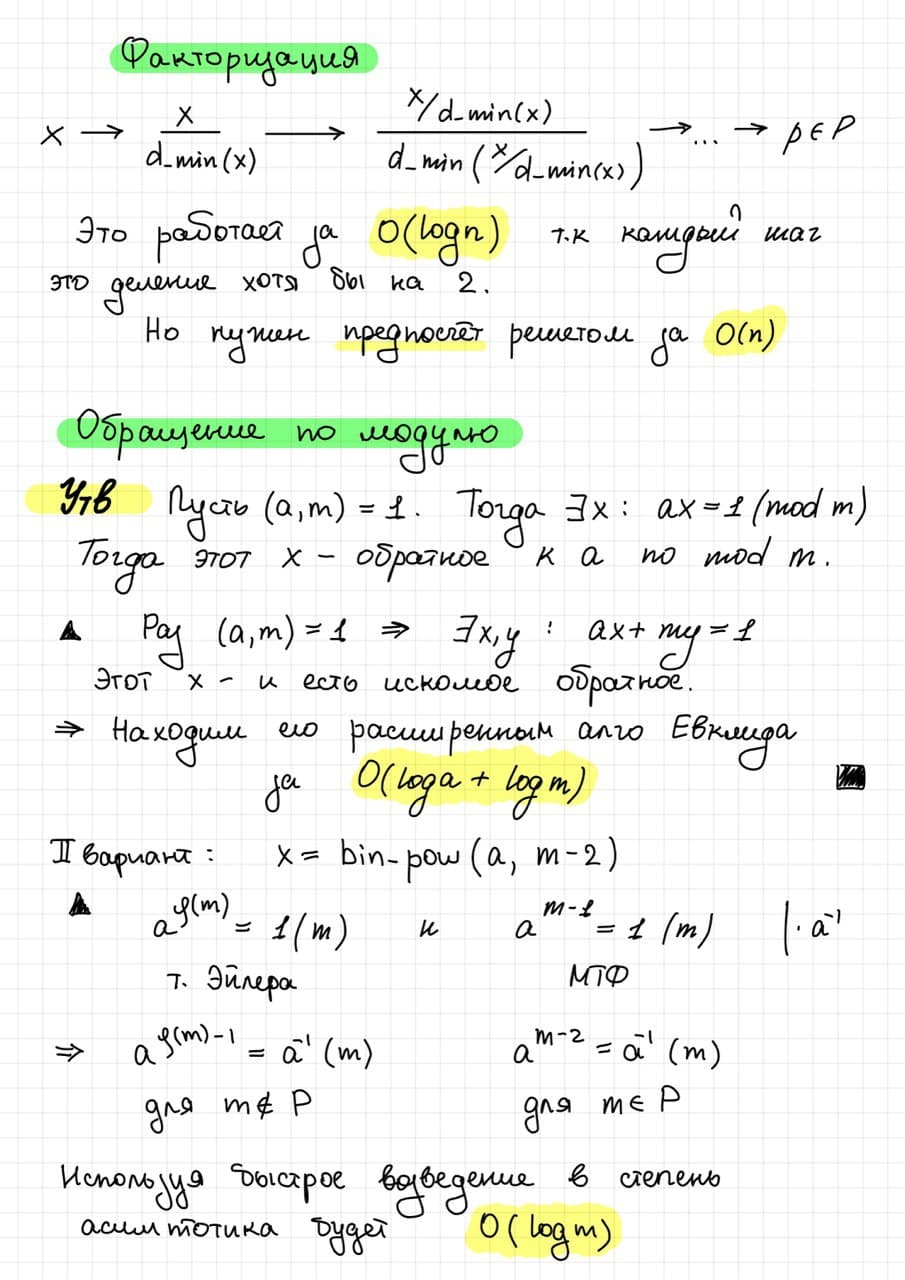
\includegraphics[width=1\linewidth]{images/mod_m.jpg}